\chapter[Background Estimation][Background Estimation]{Background Estimation}
\label{chapter:background}

The \tth multi-lepton signal regions discussed in Chapter \ref{chapter:analysis} are contaminted by background contributions at a similar order of magnitude to the signal. The dominant background for each region is vector boson production in association with top quarks (\ttV). Sub-dominant but important backgrounds include the production of vector boson pairs in associated with jets and b-quark jets (VV) and \ttbar production with a jet misidentified as a lepton (fakes). The 2l SS regions possesses a unique background of charge misidentification from Z and top events. The methods for estimating these backgrounds are discussed in this chapter. Monte Carlo simulation is used for the prompt \ttV and VV contributions. Systematic uncerainties on the overall normalization of these backgrounds in the signal region are provided from theoretical studies and past ATLAS analyses and are verified in data-based validation regions. The non-prompt backgrounds from \ttbar jet-misidentification and charge-misidentification are estimated using data-driven methods. 

For reference, Table \ref{table:background_summary} provides a summary of the \tth signal and background expectation for each of the signal regions, including the data-driven estimates discussed in this section. For each region, the background contribution exceeds the size of the signal. 


%\begin{table}
%\caption{Expected number of signal and backgroudn events in 2l SS, 3l and 4l signal regions. For data-driven backgrounds, monte-carlo only numbers are given for reference. The expected sensitivy $\frac{s}{\sqrt{s+b}}$ is provided for data-driven, mc only and for the inclusion of ad-hoc systematic uncertainties (20\% for \ttV and 30\% for \ttbar fake).}  
%\resizebox{1.0\textwidth}{!}{
%\begin{tabular}{|c|c|c|c|c|c|c|c|c|c|}\hline 
%                                       & \multicolumn{6}{c|}{Same-sign}                                         &  3 leptons    & \multicolumn{2}{c|}{4 leptons} \\
%                                       &   \multicolumn{3}{c|}{$\geq 5$ jets}  &\multicolumn{3}{c|}{4 jets}     &                  & Z enriched & Z depleted \\ \hline
%                                       &   \ee   &  \emu   & \mumu   &    \ee   &  \emu   & \mumu                &                       &  &           \\ \hline
%\bf\tth                                & $0.73\pm0.03$  &  $2.13\pm0.05$ & $1.41\pm0.04$ & $0.44\pm0.02$ & $1.16\pm0.03$& $0.74\pm0.03$ & $2.34 \pm 0.04$   & $0.19 \pm 0.01$ & $0.03 \pm 0.00$     \\ \hline
%\ttV                                   & $2.60\pm0.13$  & $7.42\pm0.17$  & $5.01\pm0.16$ & $3.05\pm0.13$ & $8.39\pm0.24$ & $5.79\pm0.20$ & $7.21 \pm 0.24$  & $0.74 \pm 0.05$ & $0.00 \pm 0.00$     \\ \hline
%tZ                                     & $$             & $$             & $$            &               &               &               & $0.71 \pm 0.03$ &   {\it incl. in \ttV}   & {\it incl. in \ttV} \\ \hline
%VV                                     & $0.48\pm0.25$  & $0.37\pm0.23$  & $0.68\pm0.30$ & $0.77\pm0.27$ & $1.93\pm0.80$ & $0.54\pm0.30$ & $0.89 \pm 0.25$ &  $0.08 \pm 0.01$ & $0.00 \pm 0.00$     \\ \hline
%\ttbar, $tX$ (MC)                      & $1.31\pm0.67$  & $2.55\pm0.84$  & $1.76\pm0.67$ & $4.99\pm1.19$ & $8.19\pm1.41$ & $3.70\pm1.03$ & $2.46 \pm 0.19$ &  $0.00 \pm 0.00$ & $0.00 \pm 0.00$     \\ \hline
%\zj (MC)                               & $0.16\pm0.16$  & $0.28\pm0.20$  & $0.12\pm0.12$ & $1.37\pm0.78$ & $0$           & $0.23\pm0.23$ & $0$             &  $0.00 \pm 0.00$ & $0.00 \pm 0.00$      \\ \hline
%fake leptons (DD)                      & $2.31\pm0.97$  & $3.87\pm1.01$  & $1.24\pm0.41$ & $3.43\pm1.38$ & $6.82\pm1.63$ & $2.38\pm0.78$ & $2.62 \pm 0.51$ &  $(1.1\pm0.6)\cdot10^{-3}$ & $(0.09\pm0.03)\cdot10^{-3}$ \\ \hline
%Q misid (DD)                           & $1.10\pm0.09$  & $0.85\pm0.08$  & $-$  & $1.82\pm0.11$            & $1.39\pm0.08$ &  $-$  & $-$             &       $-$             & $-$                  \\ \hline \hline
%Tot Background (fake MC)               & $4.56\pm1.17$  & $10.62\pm1.54$ & $7.57\pm1.31$ & $10.18\pm2.43$& $18.51\pm2.54$& $10.26\pm1.82$& $11.27 \pm 0.40$&  $0.83 \pm 0.07$ & $0.01 \pm 0.00$    \\ \hline
%Tot Background (fake DD)               & $6.49\pm1.04$  & $12.51\pm1.04$ & $6.93\pm0.52$ & $9.07\pm1.42$ & $18.53\pm1.83$& $8.71\pm0.88$ & $11.43 \pm 0.62$&  $0.831\pm 0.075$& $0.0110\pm0.0003$  \\ \hline \hline
%$s/\sqrt{b}$ (fake MC)                 & $0.34$  & $0.65$  & $0.51$  & $0.14$ & $0.27$ & $0.23$ & $0.70$      &    $0.21$  & $0.30$	  \\ \hline
%$s/\sqrt{b}$ (fake DD)                 & $0.29$  & $0.60$  & $0.54$  & $0.15$ & $0.27$ & $0.25$ & $0.69$      &    $0.21$  & $0.29$	 \\ \hline \hline
%$s/\sqrt{b} \oplus 0.3{\rm fake(MC)} \oplus 0.2{\rm ttV}$  & $0.33$  & $0.58$ & $0.47$ & $0.12$ & $0.22$ & $0.21$ &  $0.63$    & $0.207$ & $0.30$ 	 \\ \hline
%$s/\sqrt{b} \oplus 0.3{\rm fake(DD)} \oplus 0.2{\rm ttV}$  & $0.27$  & $0.53$ & $0.50$ & $0.14$ & $0.23$ & $0.23$ &  $0.62$    & $0.207$ & $0.286$	 \\ \hline
%\end{tabular}
%\label{table:background_summary}
%}
%\end{table} 


\section{Vector Boson ($W^{\pm}$, $Z$) production in association with top quarks: \ttV, \tZ}  

This section describes the estimation  and \ttV productions. 
Production of top quarks plus vector boson is an important background in all multilepton channels.   A large part of the \ttV component, arising from on-shell $Z\to\ell\ell$, can be removed via a $Z$ mass veto on like-flavour, opposite sign leptons.  However the $Z \to \tau\tau$ and $\gamma^*$ components remain. The \ttW and \tZ processes generally require extra jets to reach the multiplicity of our signal regions.  Uncertainties from the choice of the factorization ($\mu_{\rm F}$) and renormalisation $\mu_{\rm R}$ scales as well as from the PDF sets are considered evaluating their impacts on both the production cross sections and on the event selection efficiencies (particularly resulting from effects on the shape of number of jets spectrum). 

Monte Carlo events for these processes are generated with MadGraph 5 and showered with Pythia 6.  \ttW events are generated with up to two extra partons at matrix element level, while for \ttZ up to one extra parton at matrix-element level is produced.  The \tZ process is simulated without extra partons.  The next-to-leading-order (NLO) cross sections are implemented by applying a uniform $k$-factor to the leading-order (LO) events for each process.  For \ttZ, there is a large component of off-shell production, and for the 3 and 4 $\ell$ channels low mass $\gamma^*/Z \to \ell\ell$ is an important background after on-shell production is removed with a $Z$ veto.  In this case the $k$-factor is determined by comparing LO and NLO cross sections for on-shell $Z$ production only.   

The \ttV uncertainties are calculated
using the internal QDC scale and PDF reweighting that is available with
{\tt MadGraph5\_aMC@NLO}. The prescription for the scale envelope is taken from
\cite{Garzelli:2012bn}: the central value $\mu=\mu_{R}=\mu_{F}=m_t+m_V/2$
and the uncertainty envelope is $[\mu_{0}/2,2\mu_{0}]$. The PDF
uncertainty prescription used is the recipe from
\cite{Campbell:2012dh}: calculate the PDF uncertaintly using the {\tt
MSTW2008nlo}~\cite{Martin:2009iq} PDF for the central value and then the final PDF
uncertainty envelope is derived from three PDF error sets each with
different $\alpha_S$ values (the central value and the upper and lower
90\% CL values). The final NLO cross section central values and
uncertainties are given in Table~\ref{tab:ttVXSunc}.

\begin{table}%[ht!!!]
\begin{center}
\caption{NLO cross section and theoretical uncertainty
  calculations derived from {\tt MadGraph5\_aMC@NLO}.}
\label{tab:ttVXSunc}
\begin{tabular}{l|p{0.15\textwidth}|p{0.1\textwidth}|p{0.1\textwidth}|p{0.1\textwidth}|p{0.1\textwidth}|p{0.2\textwidth}}
\hline
Process & $\sigma_{NLO}$ [$fb$] & \multicolumn{2}{c|}{Scale
Uncertainty [\%]} & \multicolumn{2}{c|}{PDF Uncertainty [\%]} & Total
symmetrised uncertainty [\%] \\
\hline
\hline
$t\bar{t}W^{+}$ & 144.9 & +10 & -11 & +7.7 & -8.7 & 13.3 \\
$t\bar{t}W^{-}$ & 61.4  & +11 & -12 & +6.3 & -8.4 & 13.6 \\
$t\bar{t}Z$     & 206.7 & +9  & -13 & +8.0 & -9.2 & 14.0 \\
$tZ$            & 160.0 & +4  & -4  & +7   & -7   & 8.0 \\
$\bar{t}Z$      & 76.0  & +5  & -4  & +7   & -7   & 8.6 \\
\hline
\end{tabular}
\end{center}
\end{table}

The \tZ process is normalized to NLO based on the calculation in Ref.~\cite{Campbell:2013yla}.  Here the scales are set to $\mu_0 = m_t$ and the scale variations are by a factor of four; the scale dependence is found to be quite small.


\subsection{\ttZ Validation Region}

Unlike \ttW, a \ttZ validation region can be obtained by simply inverting the veto on same-flavor opposite sign lepton pairs near the Z pole in the 3 lepton signal region. This region thus requires 3 leptons (with momentum and identification cuts discussed in Chapter \ref{chapter:selection}, at least one opposite sign, same-flavor pair of leptons within 10 \gevcc of the Z mass, and either 4 jets and at least 1 b-tagged jet or exacly 3 jet and 2 or more b-tagged jets. The resulting region has low statistics and is not used as a control region but is instead used as a validation to demonstrate that the normalization uncertainty, discussed above, is properly evaluated. 

The region defined by this is predicted to be 67\% \ttZ, 17\% $WZ$, and 13\% \tZ.  We predict $19.3 \pm 0.5$ events and observe 28, giving a observed-to-predicted ratio of $1.45 \pm 0.27 \pm 0.03$ (where the errors are from data and simulation statistics, respectively).Given the large errors, the region is still in agreement with the predictions to within 1-1.5 $\sigma$.  Distributions of various variables are shown in Fig.~\ref{figure:background_ttZCRA}.  

\begin{figure}
 \begin{center}
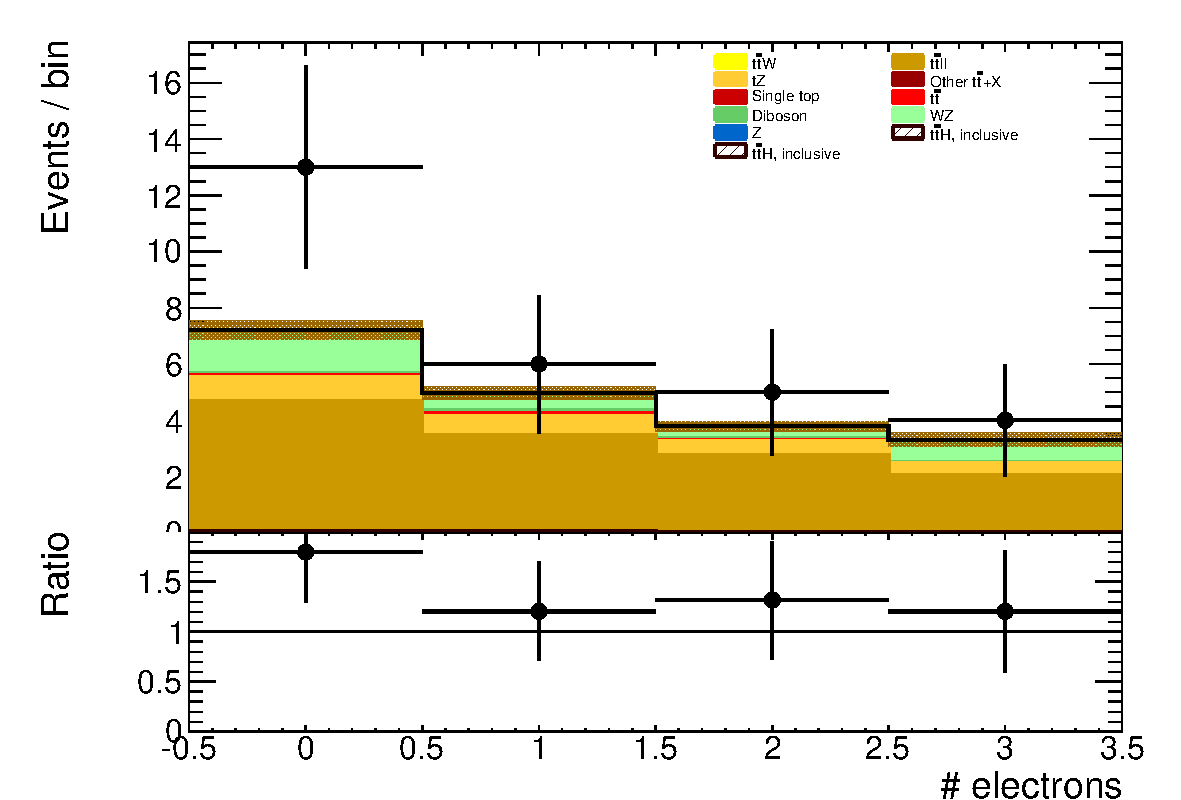
\includegraphics[width=.5\linewidth]{figs/ttZ/ttz_3l_CR_nelec}%
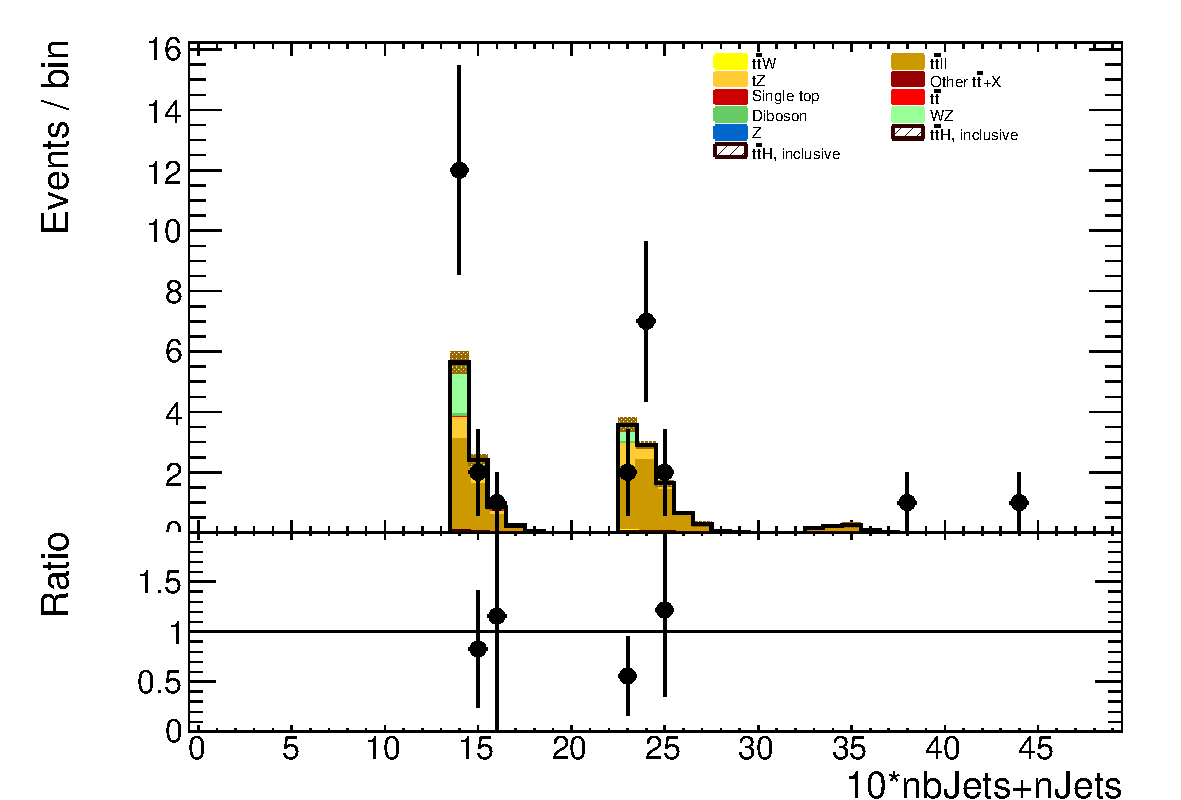
\includegraphics[width=.5\linewidth]{figs/ttZ/ttz_3l_CR_nJets_and_nbJets_lin}\\
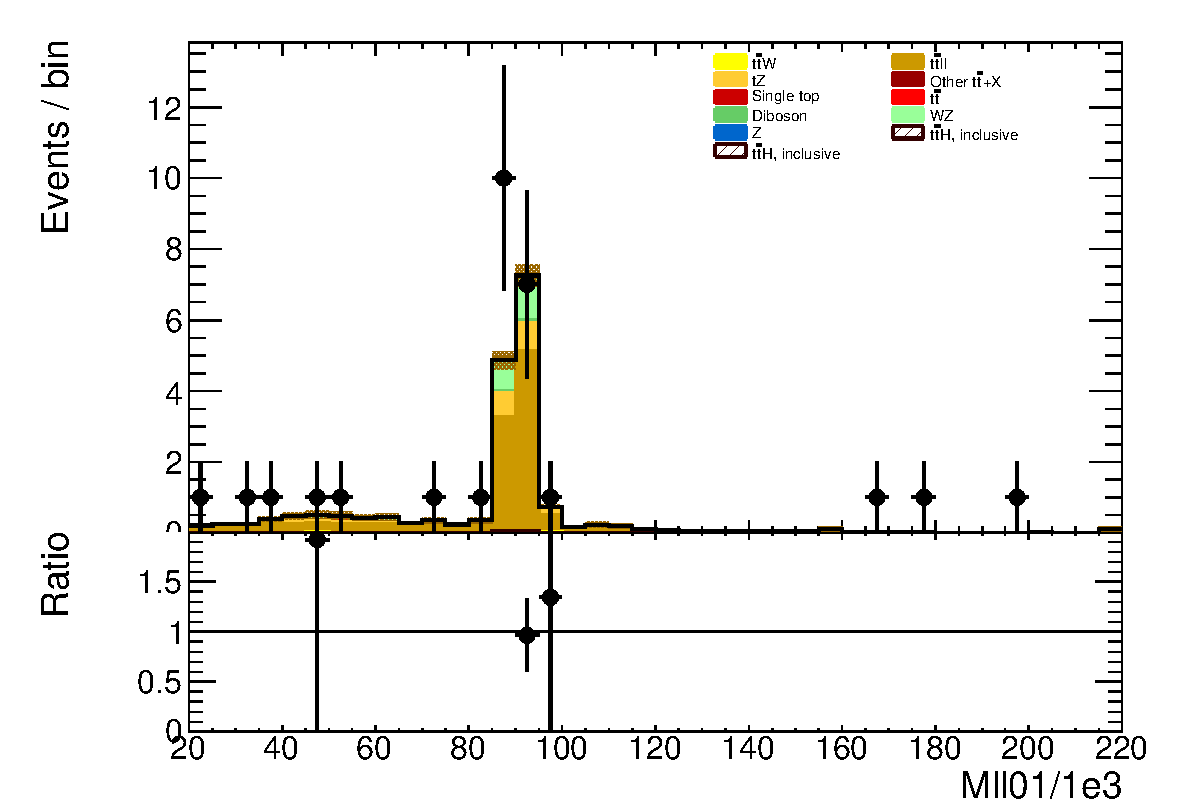
\includegraphics[width=.5\linewidth]{figs/ttZ/ttz_3l_CR_Mll01}%
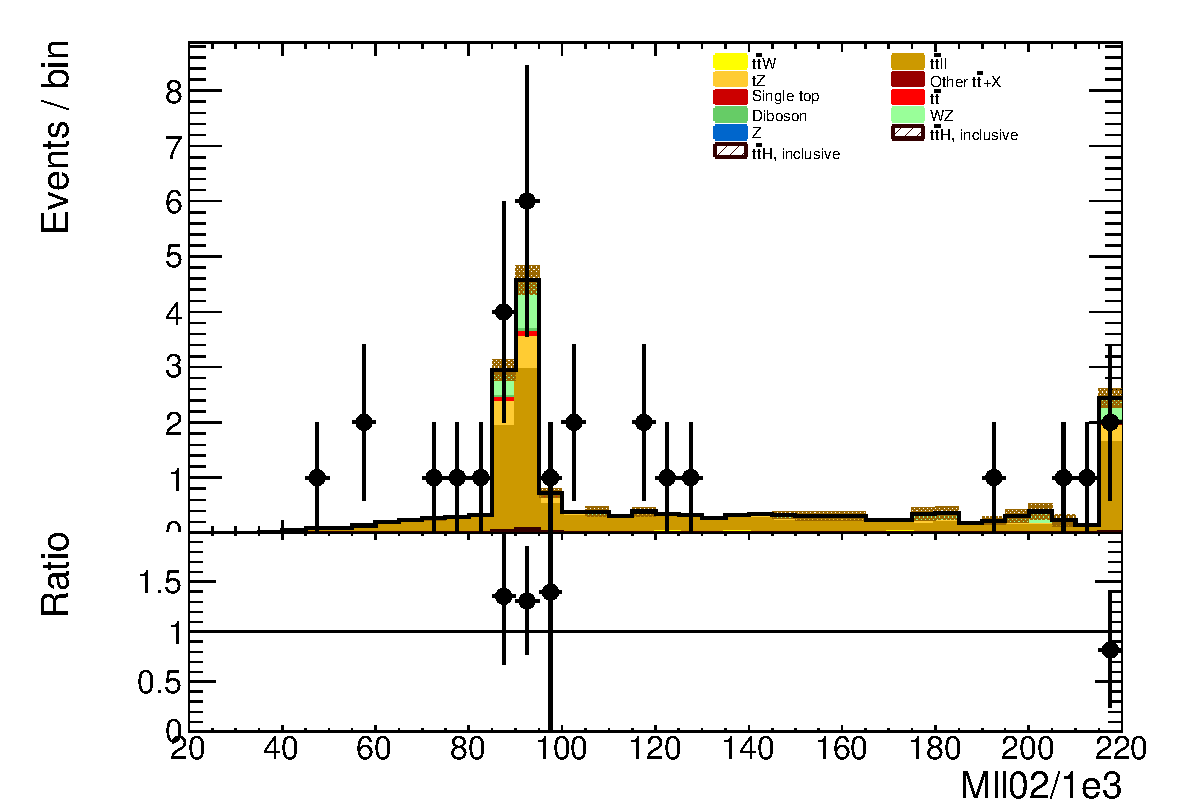
\includegraphics[width=.5\linewidth]{figs/ttZ/ttz_3l_CR_Mll02}\\
  \caption{\label{figure:background_ttZCRA}Data/MC comparison plots for \ttZ control region A ($\ge4$ jets, $\ge1$ $b$-tag and 3 jets, $\ge 2$ $b$-tag). In all plots, the rightmost bin contains any overflows.  Top left: number of electrons.  Top right: 10*the number of $b$-tags + the total number of jets. Middle left: the invariant mass of the (0,1) lepton pair (see the text for the definition of the lepton ordering).  Middle right: the invariant mass of the (0,2) lepton pair.}
 \end{center}
\end{figure}



\section{Di-boson Background Estimation: \WZ,\ZZ }

$W^{\pm}Z$ and $ZZ$ di-boson production with additional and b-tagged jets constitute small contributions to 
the 3- and 4-lepton channels respectively. In the 3-lepton case $W^{\pm}Z$ comprises $\sim$ 1 event of $\sim$ 10 
total background events while the $ZZ$ contribution accounts for approximately 10\% of the total background in the 
4-lepton channel. Because of the small size of these contributions, each of the above processes can be assigned a 
non-aggressive uncertainty based on similar previous analyses with ATLAS and cross-checked with data validation 
regions and MC truth studies. We assign an overall 50\% error on both the $W^{\pm}Z$ 3-lepton signal region 
contribution and the $ZZ$ 4-lepton signal region contribution. The details of this error assignment are discussed below.
 
Both $W^{\pm}Z$ and $ZZ$ production have been studied by ATLAS \cite{WZAtlas}\cite{ZZAtlas} but neither process
has been investigated thoroughly in association with multiple jets and b-quark jets. However, both $W+b$ \cite{WbAtlas} 
and $Z+b$ \cite{ZbAtlas} production in 7 TeV data have been shown to agree with MC models to within 20-30\%. 
A single $W$ produced in association with b-tagged jets possesses a similar topology to the $W^{\pm}Z+b$ 
process at a different energy scale and has been shown to be dominated by charm mis-tags and b-jets from gluon splitting 
and multiple parton interaction. The $W+b$ analysis unfortunately uses Alpgen MC with Herwig PS modeling and only provides
results to 1 additional jet and therefore is not directly applicable to this \tth analysis (where $W^{\pm}Z$ is modeled 
using Sherpa with massive $c$ and $b$ quarks). $Z+b$ production originates from slightly different diagrams than $ZZ+b$ 
however the sources of the b-tags are similar and the analysis above provides results with Sherpa MC with an agreement 
of $\sim$ 30\%.
 
In the following two sections the uncertainty assignments for each of these two di-boson processes will be reviewed in turn. 

\subsection{$W^{\pm}Z$ Uncertainty} 
The \tth analyses has two validation regions to test the Sherpa agreement with data for $W^{\pm}Z$: one inclusive 3 lepton region, using the three-lepton channel object and \pt\ cuts; and a $W^{\pm}Z+b$ region with 1 b-tagged jet, fewer than 4 jets (to remove \ttV), and a requirement that at least one same-flavor opposite sign pair have an invariant mass within 10 \gevcc of the Z mass. Figure \ref{figure:background_wz_incl} shows kinematic varibles for the inclusive region \footnote{the fakes are taken directly from MC}. The NJet spectrum shows good agreement within statistics across the full spectrum, giving confidence about the Sherpa high NJet SR extrapolation. Figure \ref{figure:background_wz_z_b} shows NJet spectrum for the $W^{\pm}Z+b$ validation region with good agreement in the 1 and 2 jet bins, but a slight data-MC discrepancy in the 3 jet bin. The region has low stats and around $\sim$ 60\% purity. 

We assign a conservative 50\% systematic error to cover MC modeling based on these distributions and the agreement seen in similar $W+b$ and $Z+b$ analyses and use the MC central value for the final $W^{\pm}Z$ in the SR. 

\begin{figure}[!htbp]
  \begin{minipage}[h]{0.5\textwidth}
    \centering 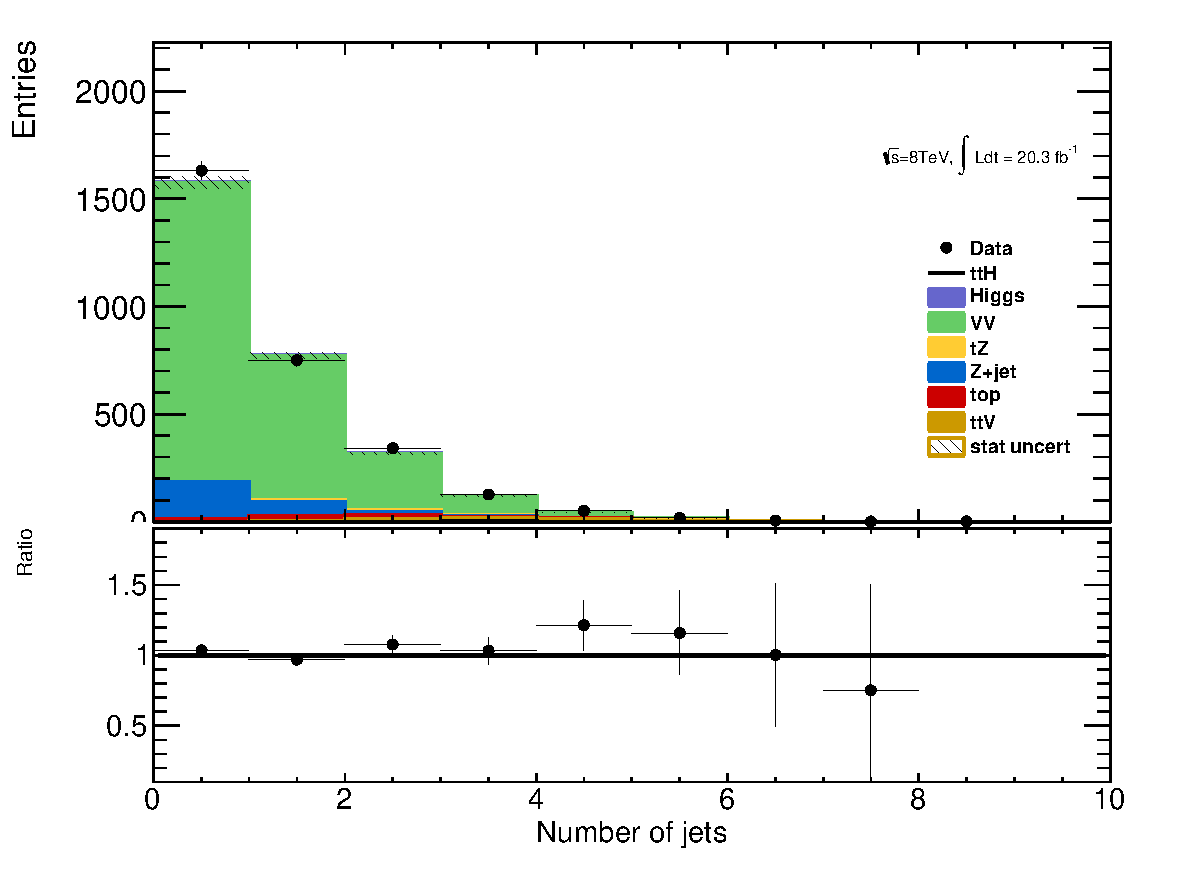
\includegraphics[width=\textwidth]{figs/WZ/plotCand_3lep_VV_NJet}
  \end{minipage}\hfill
  \begin{minipage}[h]{0.5\textwidth}
    \centering 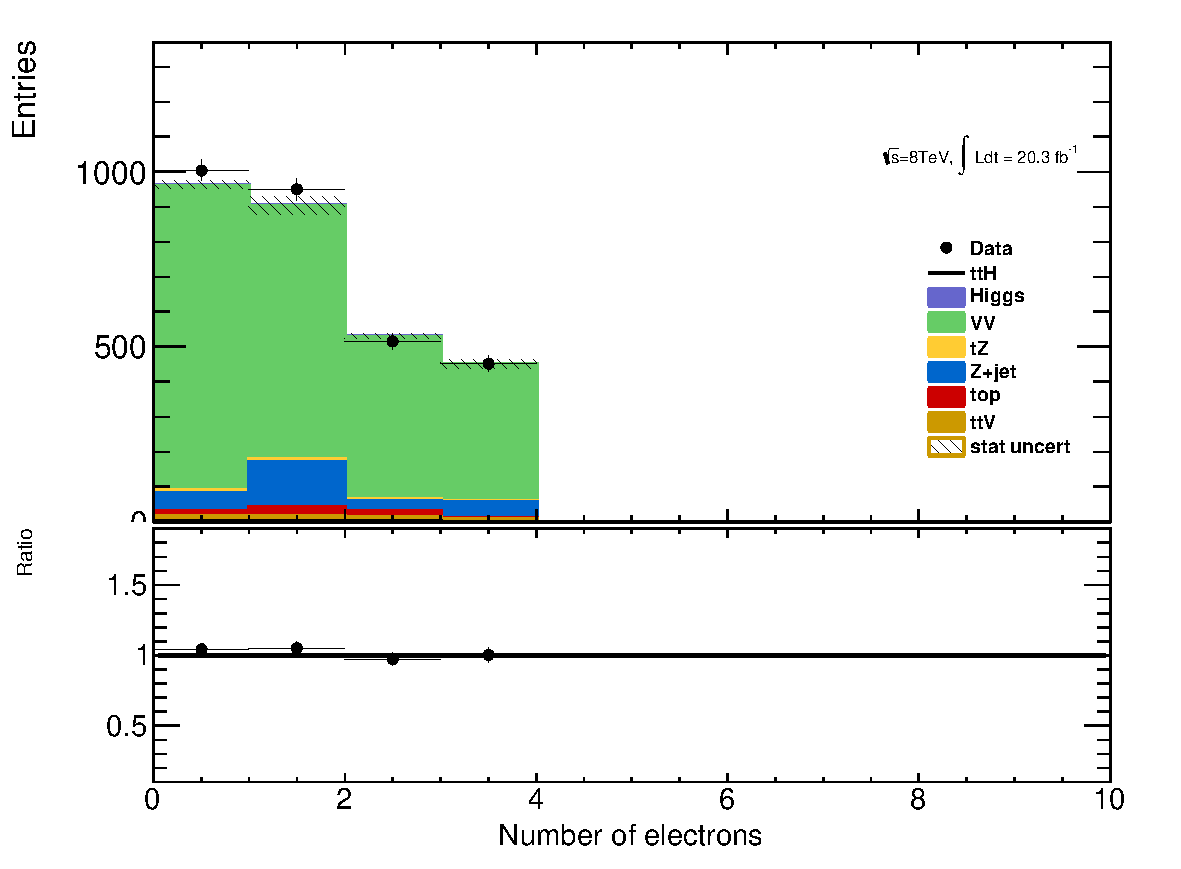
\includegraphics[width=\textwidth]{figs/WZ/plotCand_3lep_VV_NElec}
  \end{minipage}\hfill
  \begin{minipage}[h]{0.5\textwidth}
    \centering 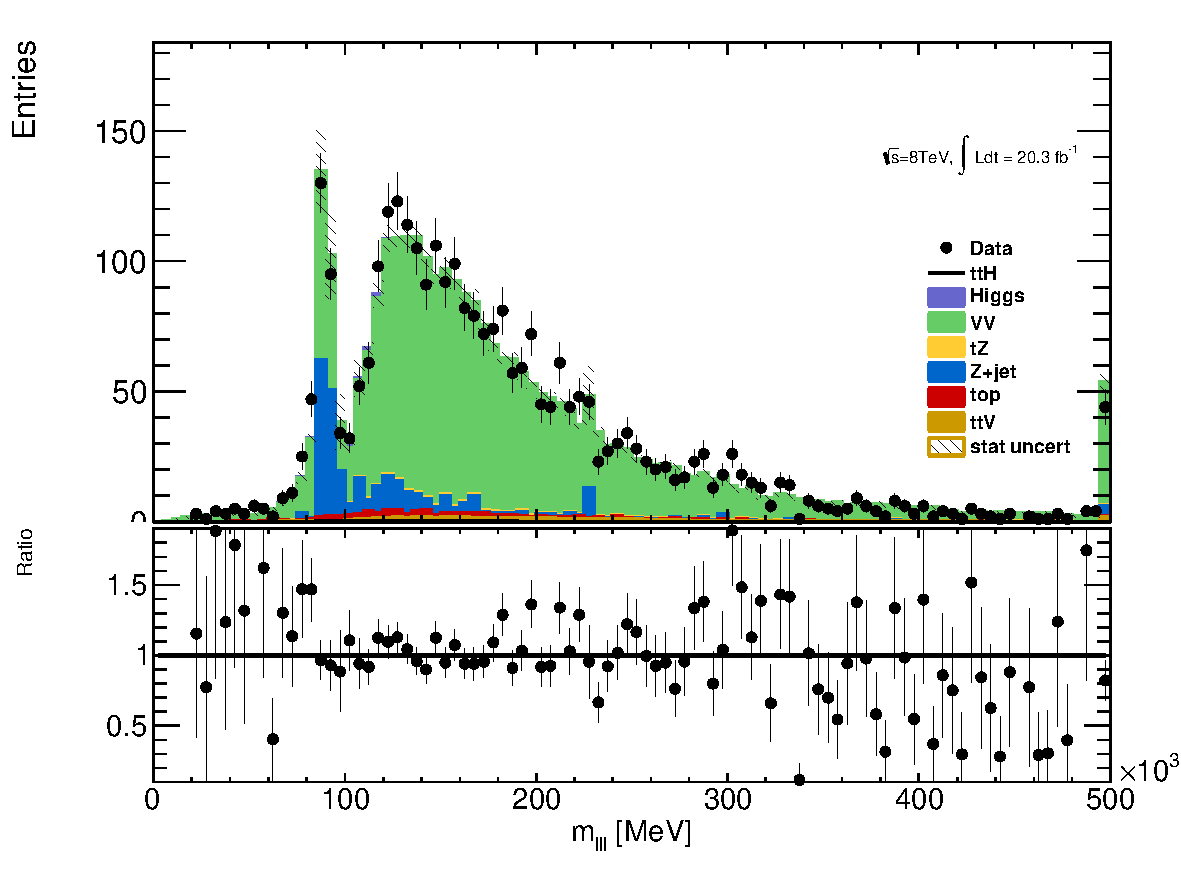
\includegraphics[width=\textwidth]{figs/WZ/plotCand_3lep_VV_Mlll}
  \end{minipage}\hfill
  \begin{minipage}[h]{0.5\textwidth}
    \centering 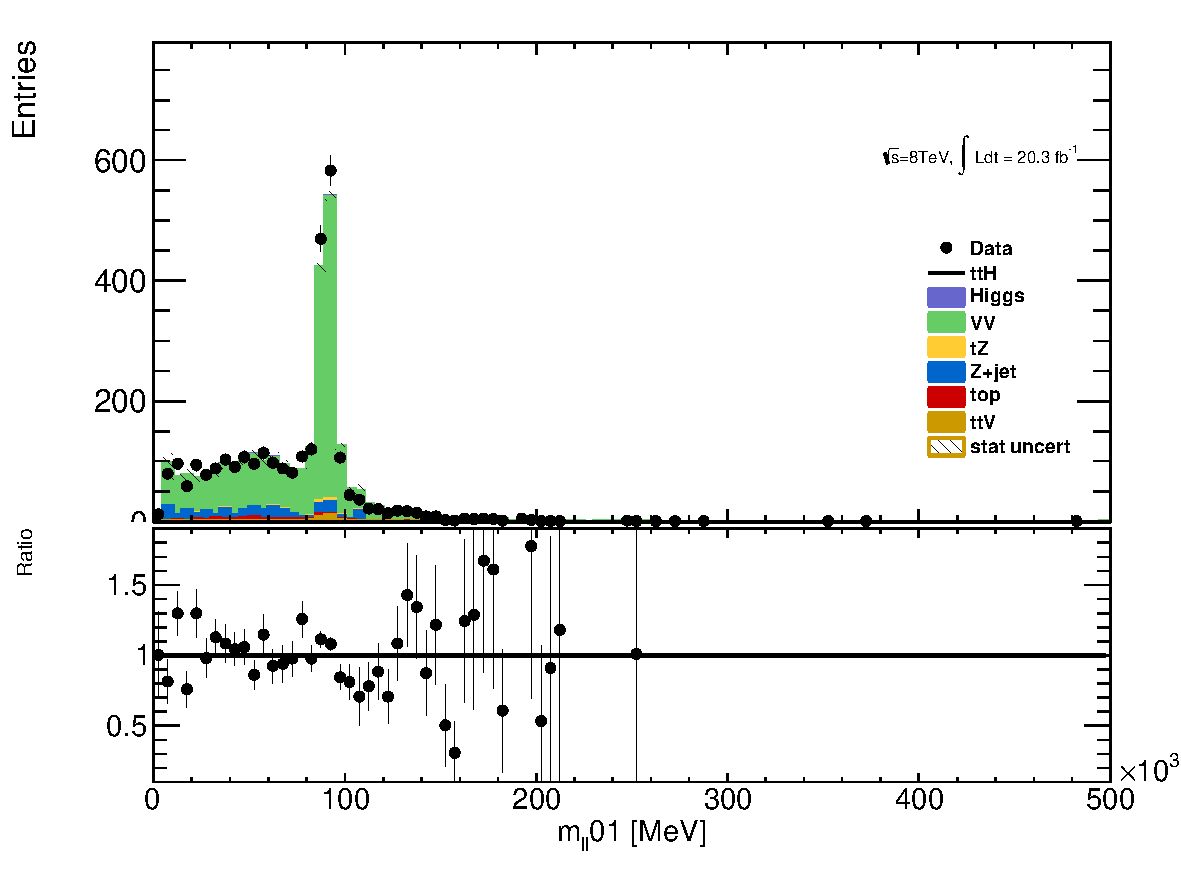
\includegraphics[width=\textwidth]{figs/WZ/plotCand_3lep_VV_Mll01ML}
  \end{minipage}\hfill

\caption{Inclusive 3 lepton $W^{\pm}Z$ validation region using the \tth lepton identification and momentum cuts: mass, number of jet and flavor variables} 
\label{figure:background_wz_incl}
\end{figure} 



\begin{figure}[!htbp]

  \begin{minipage}[h]{0.5\textwidth}
    \centering 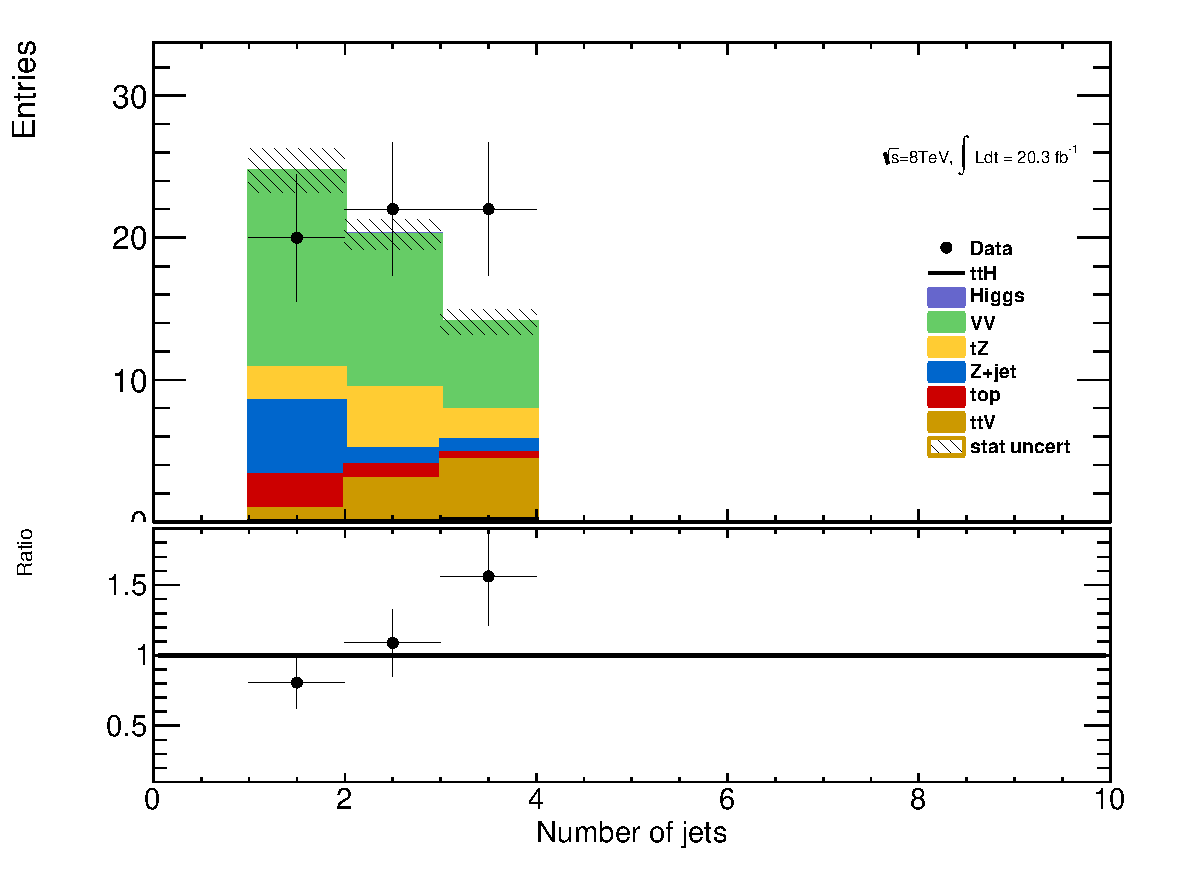
\includegraphics[width=\textwidth]{figs/WZ/plotCand_3lep_VVb_NJet}
  \end{minipage}\hfill
  \begin{minipage}[h]{0.5\textwidth}
    \centering 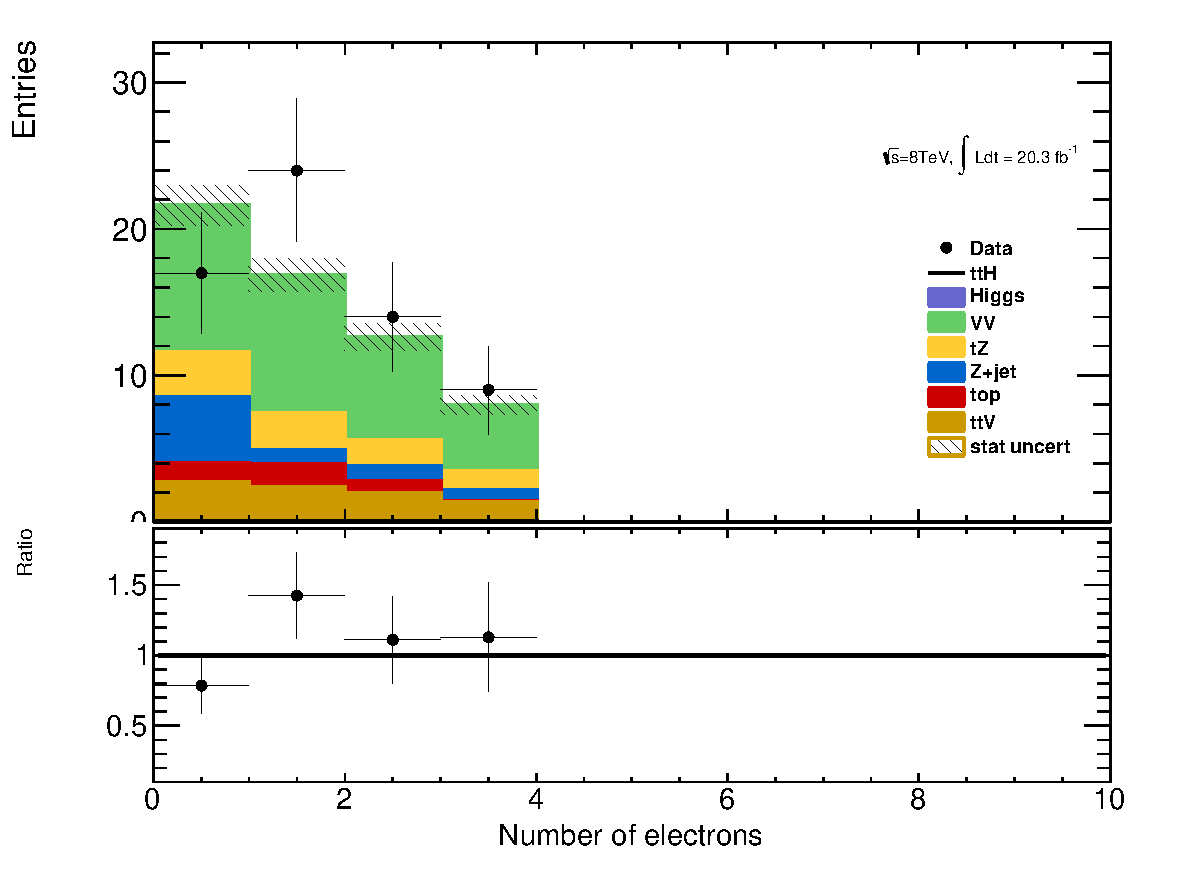
\includegraphics[width=\textwidth]{figs/WZ/plotCand_3lep_VVb_NElec}
  \end{minipage}\hfill
  \begin{minipage}[h]{0.5\textwidth}
    \centering 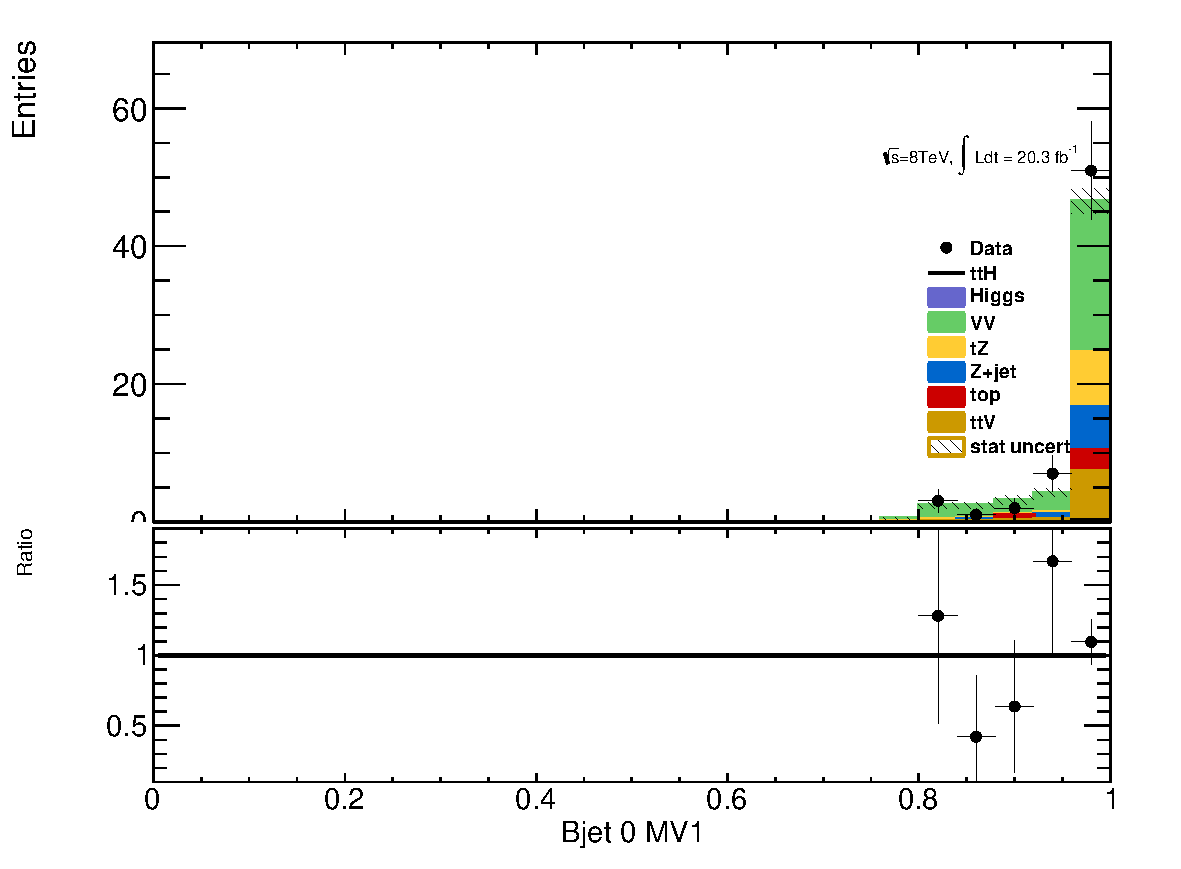
\includegraphics[width=\textwidth]{figs/WZ/plotCand_3lep_VVb_BJet0MV1}
  \end{minipage}\hfill
  \begin{minipage}[h]{0.5\textwidth}
    \centering 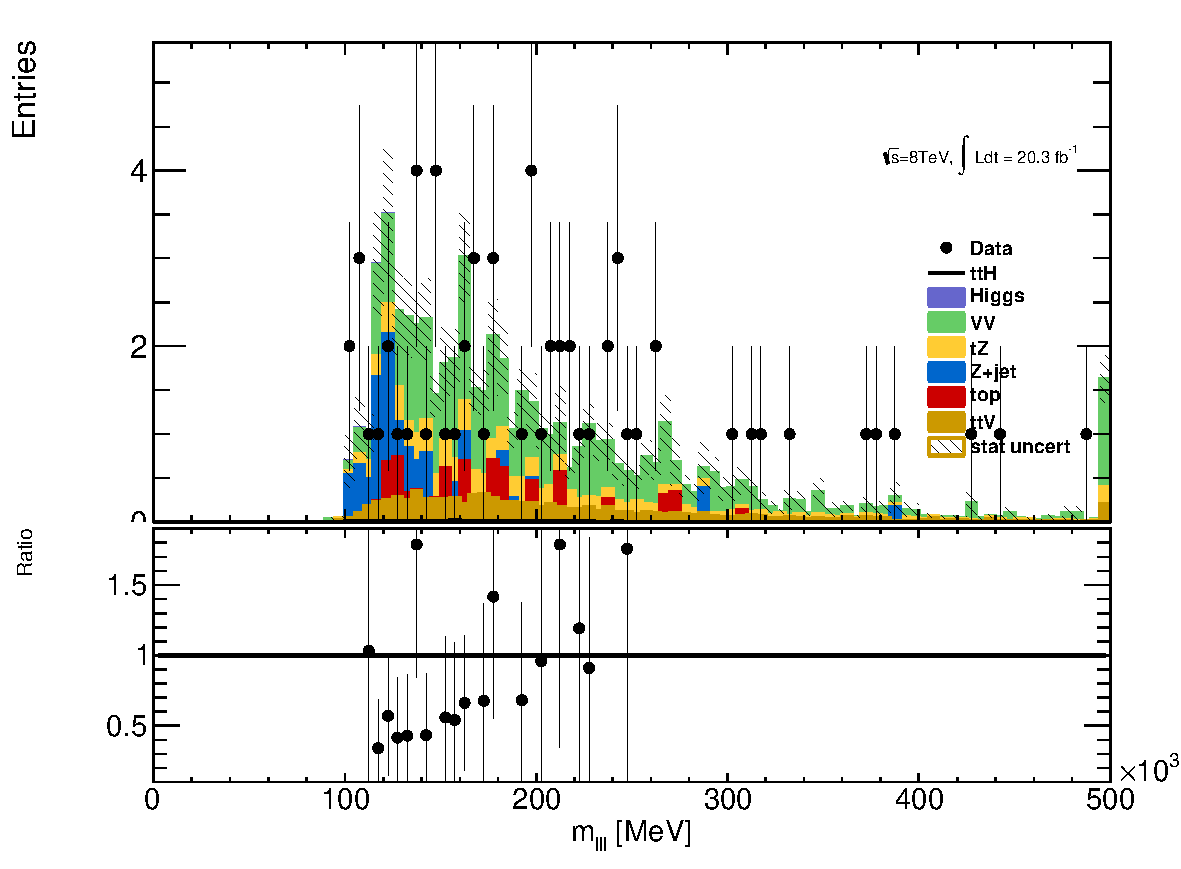
\includegraphics[width=\textwidth]{figs/WZ/plotCand_3lep_VVb_Mlll}
  \end{minipage}\hfill
\caption{$W^{\pm}Z+b$ validation region: NJet, NElec, BJet MV1 and Mass Variables} 
\label{figure:background_wz_z_b}
\end{figure} 

A cross-check is undertaken by examining the $W^{\pm}Z$ truth origins of the b-jet in the $W^{\pm}Z+b$ validation region (VR) and the signal region using the sherpa sample available. Table \ref{table:wz_truth} shows these fractions. As expected the charm and b contributions dominate, though there is a small dependence on the number of jets. The composition of the VR is fairly similar to that of the signal region, especially in the 3-jet bin. Importantly, also the tagged jet composition is also similar to the composition in the $V+b$ analysis, already measured by ATLAS and discussed above. 

\begin{table}[htbp]
\centering 
\begin{tabular}{|c|c|c|c|} 
  \hline
  & Bottom  & Charm & Light \\
  \hline
  $W^{\pm}Z+b$ VR 1 Jet& 0.25 $\pm$ 0.03 & 0.054  $\pm$ 0.04 & 0.20 $\pm$ 0.03 \\ 
  $W^{\pm}Z+b$ VR 2 Jet& 0.34 $\pm$ 0.04 & 0.052  $\pm$ 0.06 & 0.13 $\pm$ 0.03 \\ 
  $W^{\pm}Z+b$ VR 3 Jet& 0.40 $\pm$ 0.07 & 0.041  $\pm$ 0.07 & 0.18 $\pm$ 0.04 \\
  3$l$ SR              & 0.43 $\pm$ 0.14 & 0.038  $\pm$ 0.17 & 0.18 $\pm$ 0.11 \\
  \hline 
\end{tabular}
\caption{Truth Origin of highest energy b-tagged jet in the $W^{\pm}Z+b$ VR and 3$l$ SR} 
\label{table:wz_truth}
\end{table} 

\subsection{$ZZ$ Uncertainty}

In order to investigate the MC agreement with data in the $ZZ$ case, two validation regions similar to the $W^{\pm}Z$ case are defined. 
Firstly, a 4 lepton $ZZ$ region is constructed using the object selections for the 4-lepton channel and requiring exactly two pairs of 
opposite sign-same flavour leptons with a di-lepton invariant mass within 10 \gevcc of the $Z$ mass. Additionally, the $ZZ+b$ process 
is investigated directly using a similar validation region which again requires exactly two Z-candidate lepton pairs as well as at least 
1 b-tagged jet. Some kinematic distributions are shown in Figures \ref{figure:background_zz_incl} and \ref{figure:background_zz_z_b}, and particular attention should be paid to the NJet spectrum 
which shows good data-MC agreement in the high-jet bins, with a slight discrepancy in the 1-jet bin. The agreement for the region with at least 
2 jets yields confidence in the NJet MC modelling in this region which lies close to the 4-lepton signal region. 

\begin{figure}[htbp]
  \begin{minipage}[h]{0.5\textwidth}
    \centering \includegraphics[width=\textwidth]{figs/WZ/plotCand_4lep_ZZ_CR_Njet}
  \end{minipage}\hfill
  \begin{minipage}[h]{0.5\textwidth}
    \centering 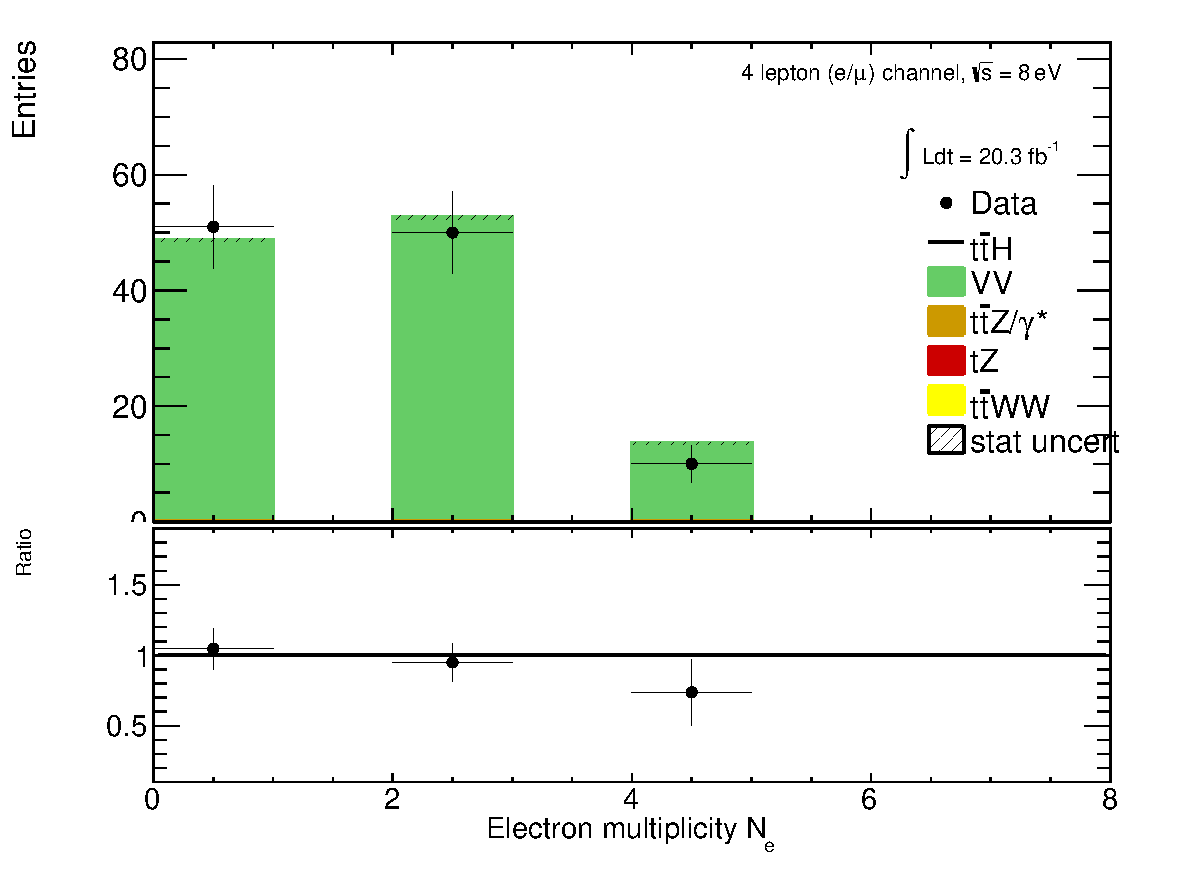
\includegraphics[width=\textwidth]{figs/WZ/plotCand_4lep_ZZ_CR_NElec}
  \end{minipage}\hfill
  \begin{minipage}[h]{0.5\textwidth}
    \centering 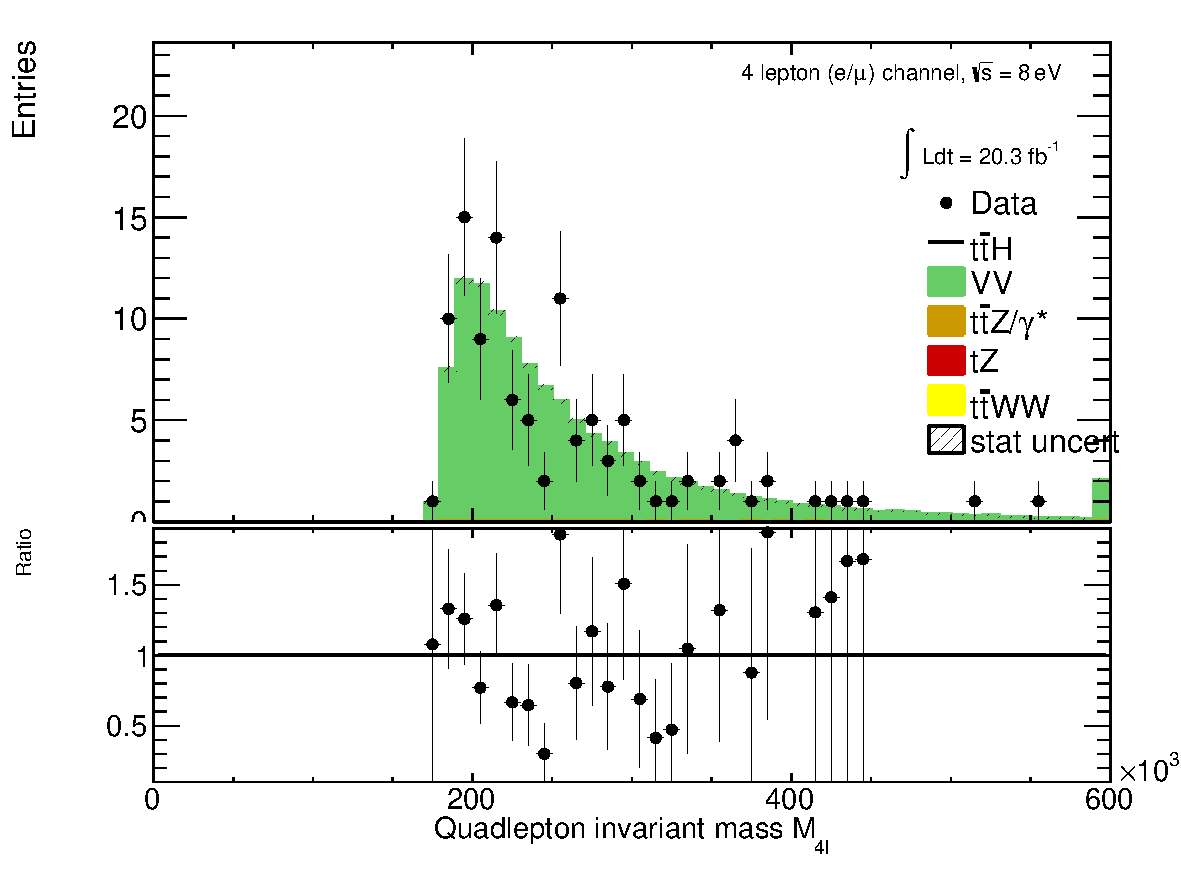
\includegraphics[width=\textwidth]{figs/WZ/plotCand_4lep_ZZ_CR_Mllll}
  \end{minipage}\hfill
  \begin{minipage}[h]{0.5\textwidth}
    \centering 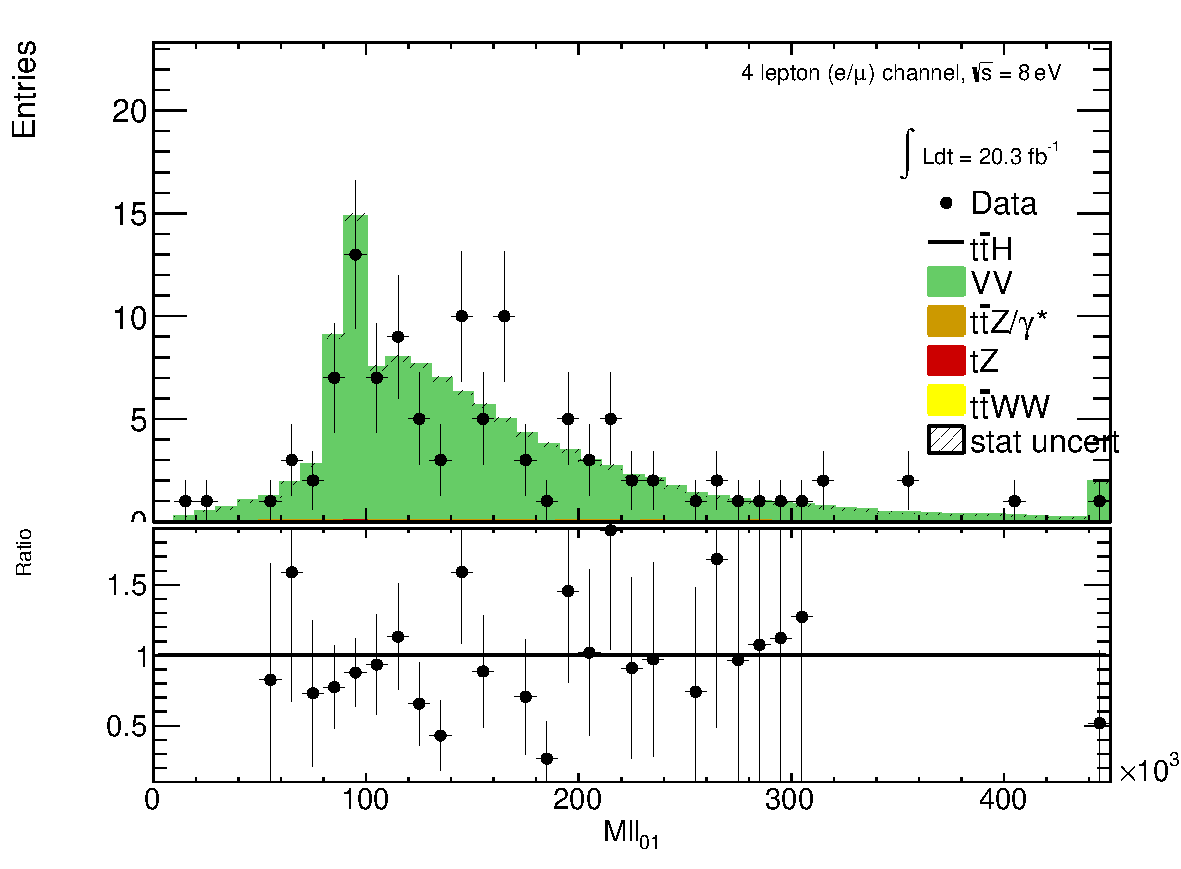
\includegraphics[width=\textwidth]{figs/WZ/plotCand_4lep_ZZ_CR_Mll01}
  \end{minipage}\hfill

  \caption{Jet-inclusive 4-lepton $ZZ$ validation region using the \tth lepton identification and momentum cuts }
  \label{figure:background_zz_incl}
\end{figure}


\begin{figure}[htbp]
  \begin{minipage}[h]{0.5\textwidth}
    \centering 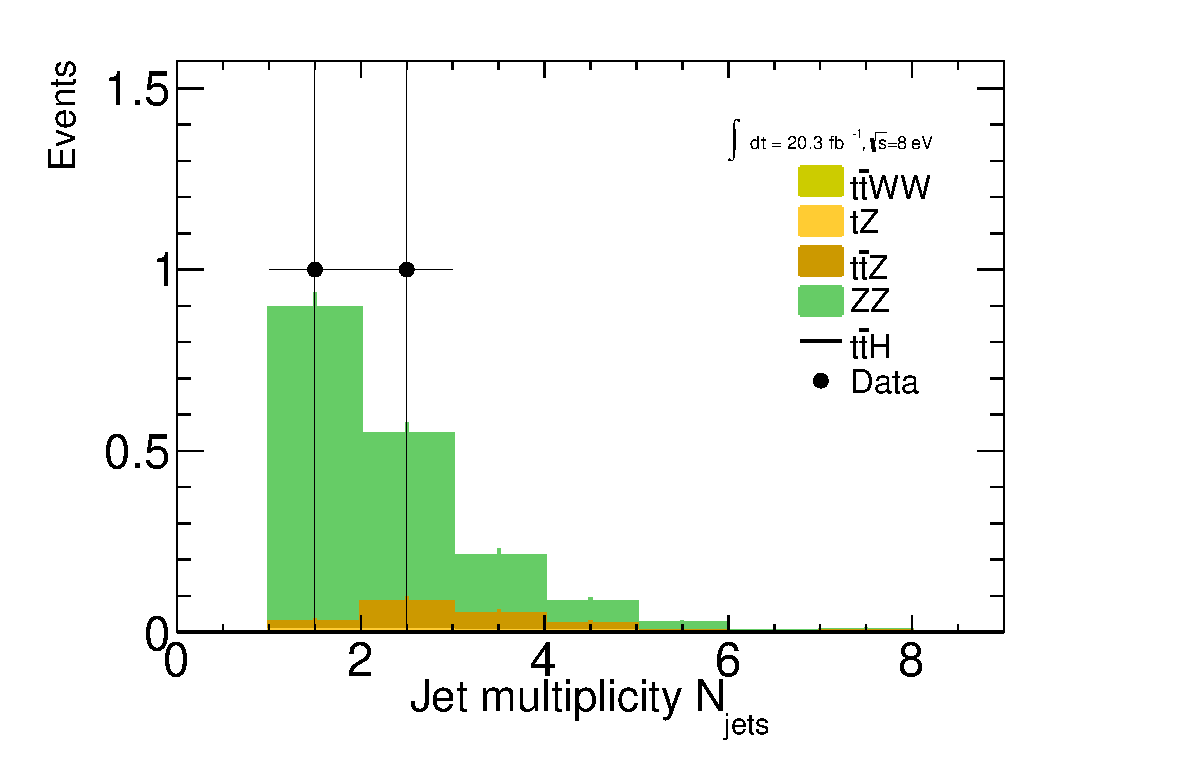
\includegraphics[width=\textwidth]{figs/WZ/zz_b_NJet}
  \end{minipage}\hfill
  \begin{minipage}[h]{0.5\textwidth}
    \centering 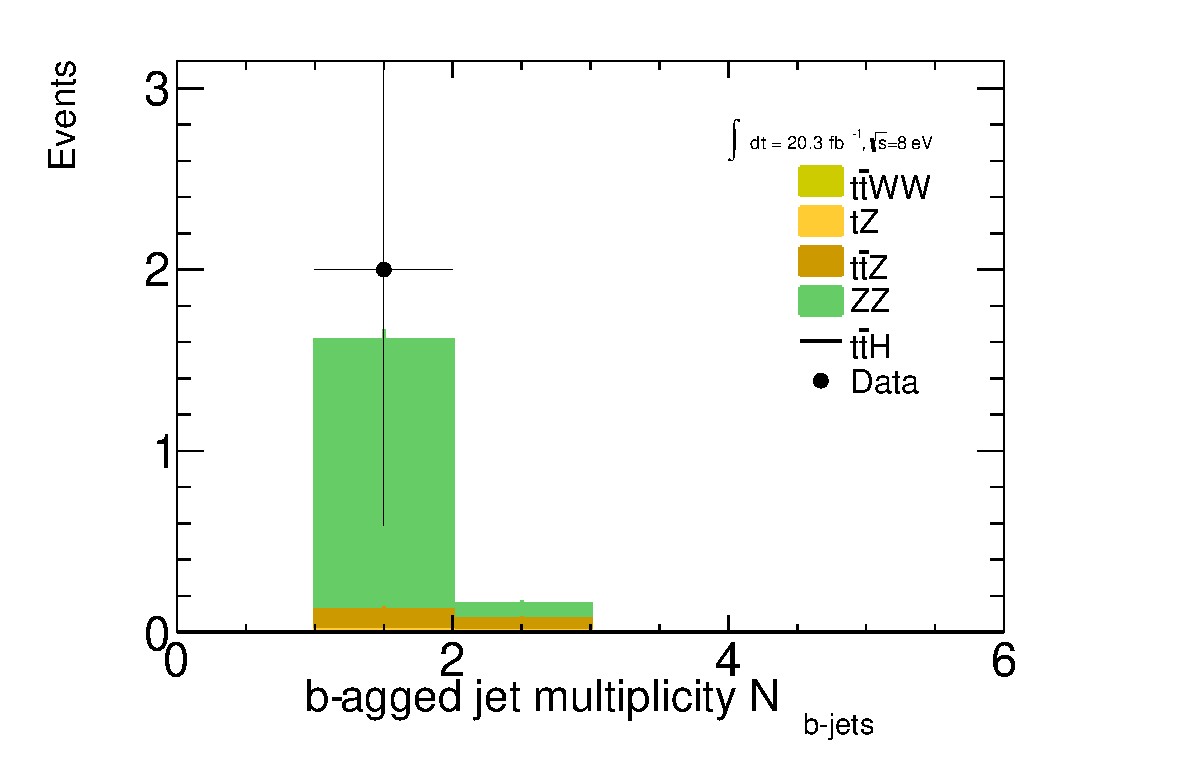
\includegraphics[width=\textwidth]{figs/WZ/zz_b_NJetBTag}
  \end{minipage}\hfill
        \caption{$ZZ+b$ validation region using the \tth lepton identification and momentum cuts }
        \label{figure:background_zz_z_b}
\end{figure}

 
Recall that in the $W^{\pm}Z$ case an overall systematic uncertainty of 50\% was assigned to cover the MC modeling. Based on the study of the $ZZ$ and 
$ZZ+b$ validation regions and the overall agreement noted with the $Z+b$ analysis, we expect a similar error to be appropriate in the $ZZ$ case.  
A similar truth origin study is undertaken in MC to demonstate a similar b-jet origin to the $W^{\pm}Z$ case. The true origin of the leading (highest energy) b-tagged jet is shown in 
Table \ref{table:zz_truth} for the 4-lepton signal region as well as the $ZZ+b$ validation region described above divided into jet bins. It can be seen 
that in case, as it was in the $W^{\pm}Z$ case above, the true origin of the b-jet in $ZZ+b$ is dominated by $c$ and $b$.

\begin{table}[htbp]
\centering 
\begin{tabular}{|c|c|c|c|} 
  \hline
                 & Bottom      & Charm       & Light \\
  \hline
  $ZZ+b$ VR 1 Jet& 0.50  $\pm$ 0.02  & 0.21  $\pm$ 0.01  & 0.18  $\pm$ 0.01 \\ 
  $ZZ+b$ VR 2 Jet& 0.25  $\pm$ 0.02  & 0.12  $\pm$ 0.01  & 0.11  $\pm$ 0.01 \\ 
  $ZZ+b$ VR 3 Jet& 0.085 $\pm$ 0.014 & 0.040 $\pm$ 0.011 & 0.036 $\pm$ 0.011 \\
  4$l$ SR        & 0.020 $\pm$ 0.008 & 0.025 $\pm$ 0.008 & 0.014 $\pm$ 0.005 \\
  \hline 
\end{tabular}
\caption{Truth Origin of highest energy b-tagged jet in the $ZZ+b$ VR and 4$l$ SR} 
\label{table:zz_truth}
\end{table} 


\section{Charge-Misidentification Background }

Charge-misidentification contributes to the background for 2l SS case and only for flavor channels, which include electrons. The same-sign require is useful in removing large SM opposite sign-backgrounds, but because of their size even small charge mis-identification rates result in contamination in same-sign regions. For the 2l SS signal regions and low NJet control regions, charge-misidentification backround arise primarly from \ttbar di-lepton events with a smaller contribution from leptonic $Z$ decays. 

In general, charge-misidentification can arise in two ways. The first occurs for ultra-high energy electrons and muons, which leave tracks in the detector that are too straight for the fit detetermine the direction of curvature with high confidence. This type of charge mis-identification is not a concern to the \tth multi-lepton analysis, as most of the leptons have momentum $>$ 150 \gevc. The second source of charge misidentification is from 'tridents', which only occurs for electrons, because their low mass allows for high rate bremmstrahlung in the detector material. In some cases, after an electron releases a photon through bremstrahlung, the photon may convert nearby resulting in three electron tracks. The reconstruction algorithms may sometimes match the wrong track to the calorimeter energy deposit, resulting in a possible charge mis-identifcation. As discussed in the selection, tight track-cluster geometric and energy matching requirements are applied on the electron candidates to reduce the overall rate and the electron acceptance is narrowed to ($|\eta| < 1.37$), since most of the material is concentrated more forward in the detector. For this reason, muon charge-misidentification is considered neglibible for this analysis.

We estimate the contribution of charge-misidentification events in our 2l SS signal regions and relevant control regions by appling a weight per electron in the opposite-sign region with otherwise same cuts. The weight is related to the charge-misidentification rates and is estimated using a likelihood method in the opposite-sign and same-sign $Z\rightarrow ee$ control regions. The rate measured from these control regions is binned in electron \pt and $\eta$, to account for dependencies in these variables. The method, validations and associated errors are discussed in detail in the following sub-sections.


\subsection{Likelihood Method}

The number of reconstruted same-sign ($N_{ss}$) and opposite sign ($N_os$) $Z\rightarrow ee$ events are related to number of produced $Z\rightarrow ee$ opposite sign events ($N$) via factors related to the charge mis-identification rate. For a single per-electron charge mis-identification rate ($ilon$, these quantities are related as follows (with the assumption that $ilon$ is very small: 

\begin{itemize}
\item $N^{os} = (1-2ilon+2ilon^2) N$ opposite-sign events,
\item $N^{ss} = 2ilon(1-ilon) N \simeq 2ilon N$ same-sign events,
\end{itemize}


Knowing $ilon$, the charge-misidentification rate, and supposing we can have a different rate per-electron, it is possible to estimate the number of same-sign events from the number of opposite sign events.

\begin{itemize}
\item $N^{ss} = \frac{ilon_i +ilon_j -2ilon_i ilon_j}{1-ilon_i -ilon_j +2ilon_i ilon_j} N^{os}$ for the $ee$ channel,
\item $N^{ss} = \frac{ilon}{1-ilon} N^{os}$ for the $e\mu$ channel,
\end{itemize}
where $ilon_i$ and $ilon_j$ are the charge mis-identification rates for the two
different electrons.


Althought it is impossible from a typical same-sign $Z\rightarrow ee$ to know which electron's charge was mis-identified, we can use a likelihood method over the whole sample to measure charge mis-identification rate ($ilon$) depends on the electron \pt and \eta.  The likelihood method assumes that  the mis-identification rates of the electron charge are independent for different pseudorapidity regions. Therefore, the probability to have a number of same-sign events ($N^{ij}_{ss}$) with electrons in $|\eta|$ region $i$ and $j$ can be written as a function of the number of events $N^{ij}$ as follows:
\begin{equation}
N^{ij}_{ss}=N^{ij}(ilon_i+ilon_j).
\end{equation}


If all the same-sign events in the $Z$ peak are produced by charge mis-identification, then $N^{ij}_{ss}$ is described by a Poisson distribution:
\begin{equation}
f(k,\lambda)=\frac{\lambda^k e^{-\lambda}}{k!},
\end{equation}
where $k$ is the observed number of occurrences of the event, i.e. $k=N^{ij}_{ss}$, and $\lambda$ is the expected number,  i.e. $\lambda=N^{ij}(ilon_i+ilon_j)$. Thus, the probability for both electrons to produce a charge mis-identification is expressed by:
\begin{equation}
P(ilon_i,ilon_j|N^{ij}_{ss},N^{ij})=\frac{[N^{ij}(ilon_i+ilon_j)]^{N_{ss}^{ij}}e^{-N^{ij}(ilon_i+ilon_j)}}{N^{ij}_{ss}!}.
\end{equation}

The likelihood $L$ for all the events is obtained by evaluating all the $|\eta|$ combinations:

\begin{equation}
L(ilon|N_{ss},N)=\prod_{i,j}\frac{[N^{ij}(ilon_i+ilon_j)]^{N_{ss}^{ij}}e^{-N^{ij}(ilon_i+ilon_j)}}{N^{ij}_{ss}!},
\end{equation}
where the rates $ilon_i$ and $ilon_j$ can be obtained by minimizing the likelihood function. In this process, the $-\ln L$ is used in order to simplify and make easier the minimization. Terms which do not depend on the rates $ilon_i$ and $ilon_j$ are removed in this step. This way, the final function to minimize is given by the following expression:
\begin{equation}
\label{eq:like}
-\ln L(ilon|N_{ss},N)\approx \sum_{i,j}\ln[N^{ij}(ilon_i+ilon_j)]N^{ij}_{ss}-N^{ij}(ilon_i+ilon_j).
\end{equation}

The events are selected within the $Z$ peak and stored --with the electron order by $|\eta|$-- in two triangular matrices: one for the same-sign events $N^{ij}_{ss}$,  and the other one for all events $N^{ij}$. The likelihood method takes into account
electron pairs with all $|\eta|$ combinations, which allows to use the full available statistics  getting therefore lower statistical uncertainties. Moreover, it does not bias the kinematical properties of the
electrons, compared to other methods like tag-and-probe.

The likelihood  method can be easily extended to measure the charge mis-identification rates as a function of  two parameters. In this study, the interest lies not only on the measurement of the rates   as a function of the pseudorapidity, but also transverse momentum. Thus, the probability to find a same-sign event given the rates for each electron is ($ilon_{i,k}+ilon_{j,l}$), where the two indices represent binned $|\eta|$- and $p_{\rm T}$-dependence. Thus, the Eq.~\ref{eq:like} transforms into
\begin{equation}
-\ln L(ilon|N_{ss},N)\approx \sum_{i,j,k,l}\ln[N^{ij,kl}(ilon_{i,k}+ilon_{j,l})]N^{ij,kl}_{ss}-N^{ij,kl}(ilon_{i,k}+ilon_{j,l}).
\end{equation}   

The likelihood method uses only $Z$ $signal$ events. Therefore, background coming from other processes where the dilepton invariant mass corresponds to the one of the $Z$ boson needs to be subtracted. The background subtraction is done using a simple side-band method.   This method consists in dividing the $Z$ invariant mass in three regions, i.e. $A$, $B$ and $C$, where $B$ is the central region corresponding to the $Z$ peak. The number of events is counted in the regions on the sides of the peak, i.e. $n_A$ and $n_C$, and removed  from the total number of events in the peak region $B$, $n_B$. This way, the number of signal events $N_Z$ is given by
\begin{equation}
N_Z=n_B-\frac{n_A+n_C}{2}.
\end{equation}
  
 Once the background has been subtracted, the likelihood method can be applied. {\tt MINUIT} is used for the minimization and {\tt MIGRAD} to compute the uncertainty on these rates. 


\subsection{Results}

The charge mis-identification rate is calculated in 7 $|\eta|$ bins [0.0, 0.6, 1.1, 1.37, 1.52, 1.7, 2.3, 2.47] by 4 \pt bins [15,60,90,130,1000]. For \pt bins above 130 \gevc, the $Z$ dataset becomes too small and the rates are calculated using \ttbar MC, scaled by the data-MC ratio of the rates in the lower \pt bins, [90-130] \gevc. Figure \ref{figure:background_cf} shows the extracted rates in all bins.

\begin{figure}[ht!]
\centering
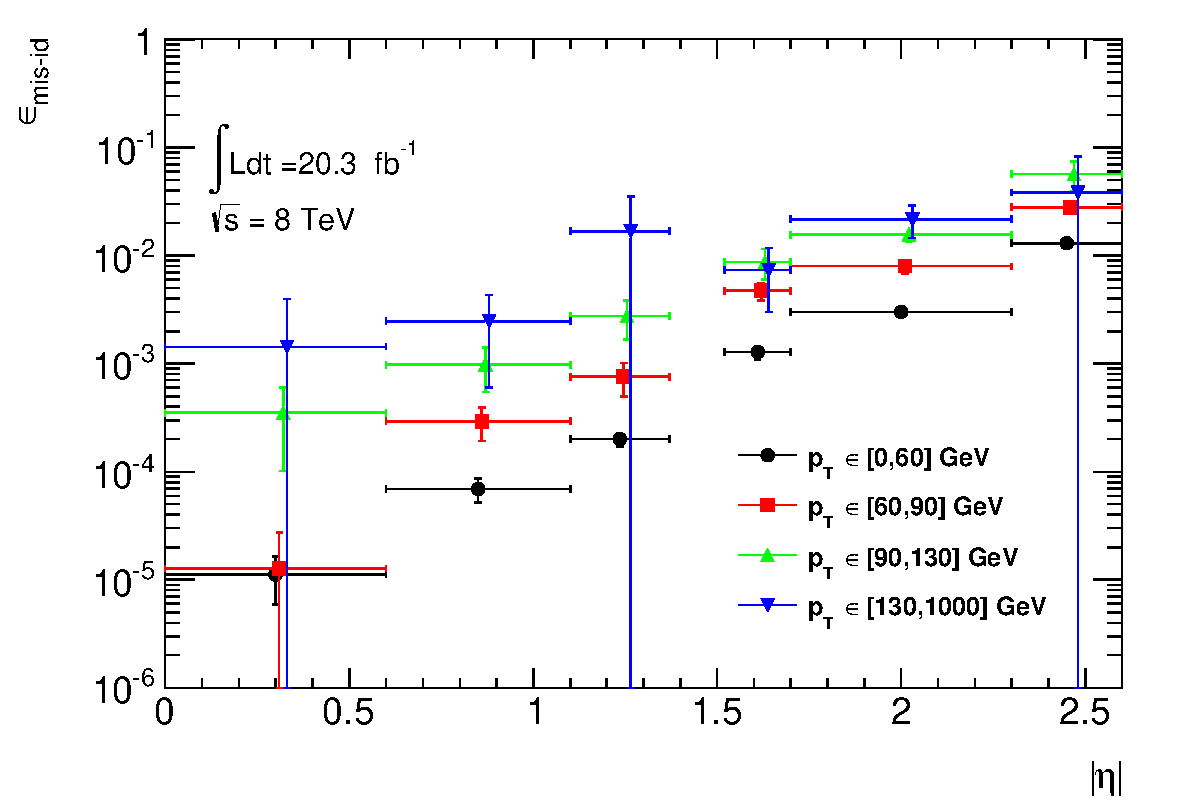
\includegraphics[width=0.7\textwidth]{figs/qmis/Rates2D}
  \caption{Electron charge mis-identification rates  measured in data with the likelihood method  on $Z$ events (black points, red squares and blue triangles) as a function of $|\eta|$ and parametrized in $p_{\rm T}$. The full 2012 dataset has been used to estimate the rates below 130~GeV.   Above this value, the charge mis-identification rates have been estimated by extrapolating the rates in the region where the $p_{\rm T}\in[90,130]$~GeV with a $p_{\rm T}$ dependent factor extracted from simulated $t\bar t$ events (green triangles). Statistical and systematic uncertainties  have been included in this plot. \label{figure:background_cf}}
\end{figure}


To validate the likelihood approach, we apply the full method to the $Z$ MC samples (extracting rates via a likelihood fit and applying them to opposite sign events) and compare to the MC predicted number of same-sign events. The invariant mass of the $Z$ from our charge mis-identification and directly from the MC can be seen on Figure~\ref{figure:background_clMll}. In the simulated $Z$ samples, the number of same-sign $Z$ events is $5~049$ while the estimation is $5~031^{+375}_{-365}$.  The uncertainties combine both statistical systematic uncertainties, which are discussed in depth below. The validation gives compatible results within uncertainties. 
 
\begin{figure}[htb!]
\centering
\begin{minipage}[h]{0.5\textwidth}
    \centering 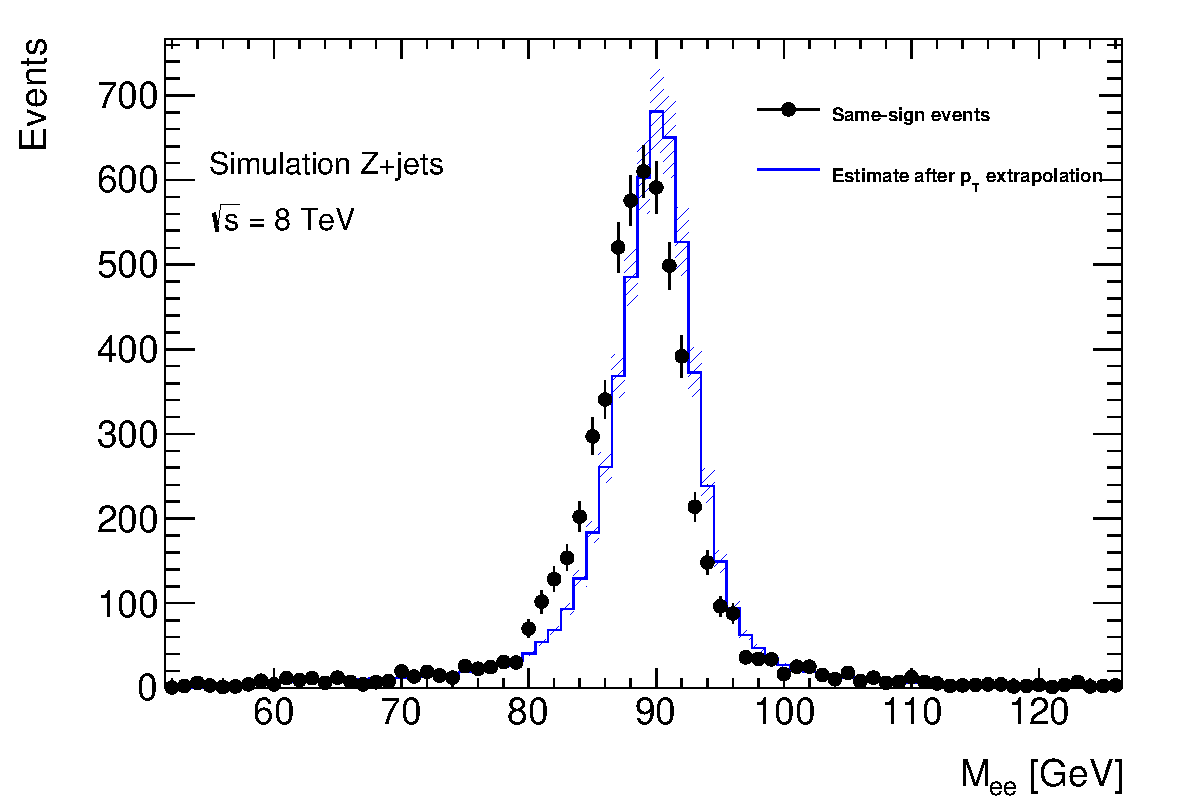
\includegraphics[width=\textwidth]{figs/qmis/ClosureMllMC}
\end{minipage}\hfill
\begin{minipage}[h]{0.5\textwidth}
    \centering 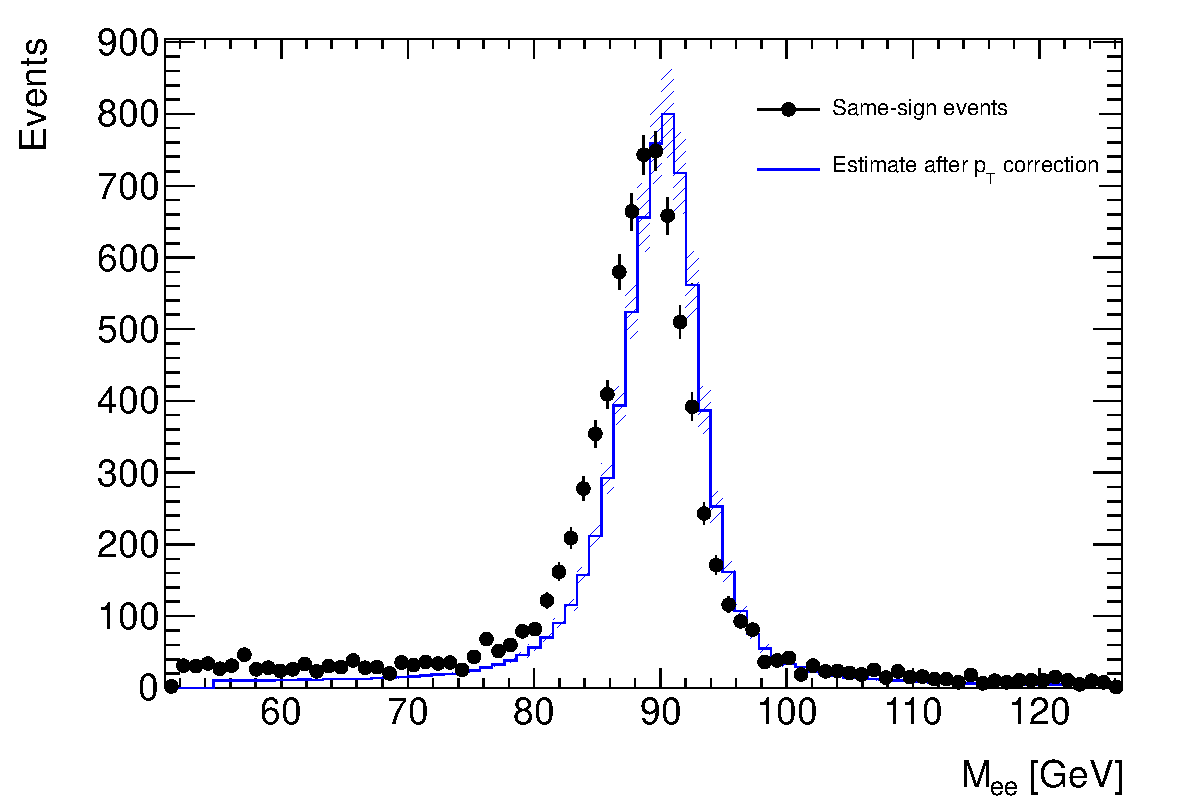
\includegraphics[width=\textwidth]{figs/qmis/ClosureMlldata}
\end{minipage}\hfill
  \caption{Closure test on simulated $Z\rightarrow e^+e^-+jets$ events (a)   and data (b). 
      The black circles show the distribution of same-sign events while the blue histograms
      show the distribution of the reweighted opposite-sign events together with the statistical and systematic uncertainties. The distributions are not
    expected to overlay exactly, due to the loss of energy of the trident electrons for the
    same-sign peak. \label{figure:background_clMll}}
\end{figure}


\subsection{Systematic and Statistical Uncertainties}

Statistical uncertainties dominate the combined uncertainty on the charge mis-identification estimate. The statistical uncertainties come primarly from the size of the $Z$ same-sign sample in data and are especially large for central, material-poor regions where the charge mis-identification rate is extremely low. Additionaly systematic uncertainties are included for a comparison between the positron and electron rate, the per-bin MC closure test discussed above in the Results section, and for the effect of varying the invariant mass window used for the background subtraction for three different cases. The high \pt extrapolation induces a statistical error only in the last \pt bin. This bins is essentially irrelevant to the energy scales considered in this analysis. Figure \ref{figure:background_qmissyst} shows the relative bin uncertanties for all rate bins.



 \begin{figure}[htp!] 
\centering
\setlength{\fboxrule}{0 pt}
\fbox{  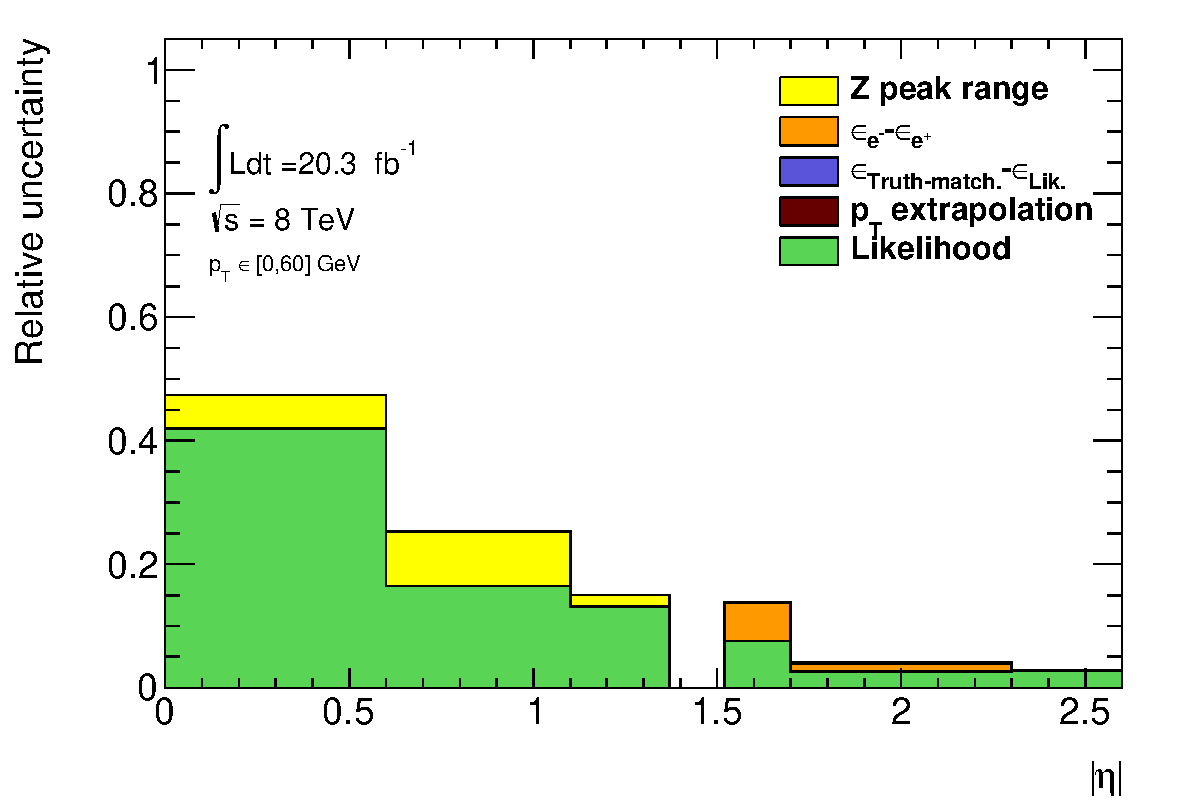
\includegraphics[width=0.48\textwidth]{figs/qmis/Syst1}}% \hspace{2cm}%
\fbox{  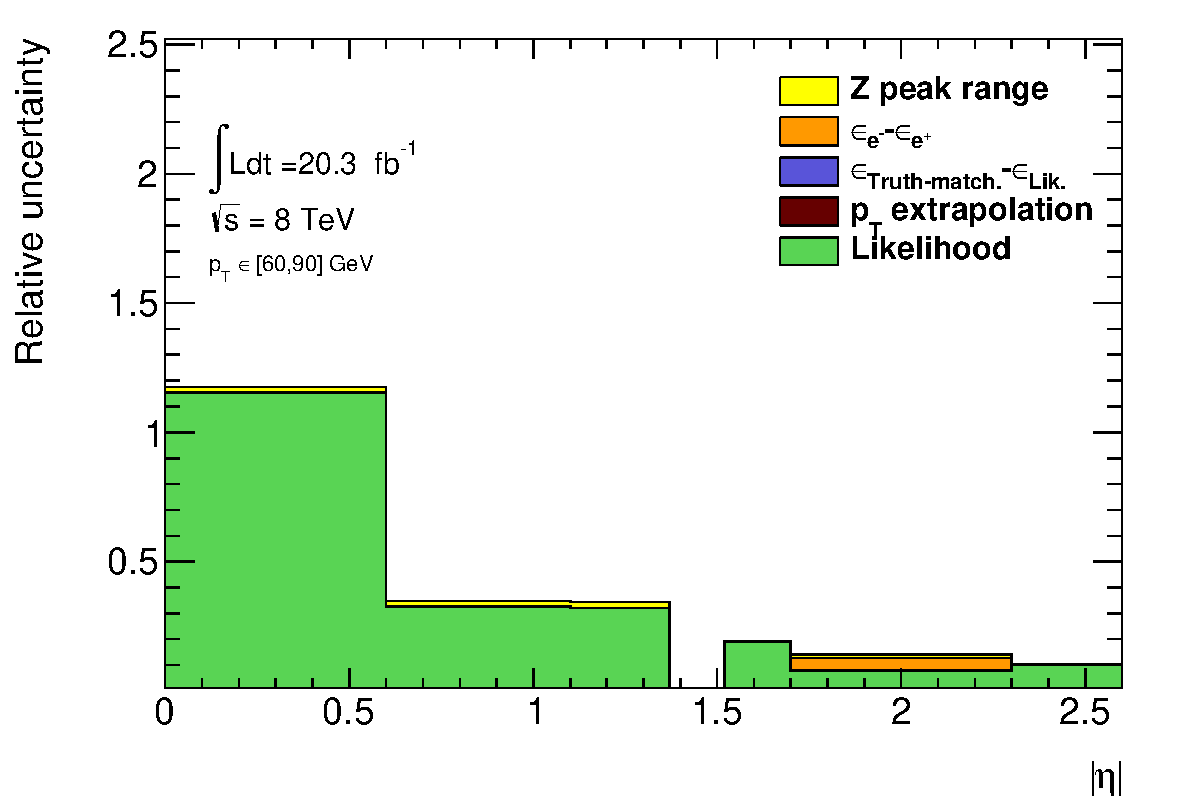
\includegraphics[width=0.48\textwidth]{figs/qmis/Syst2}}% 

\fbox{  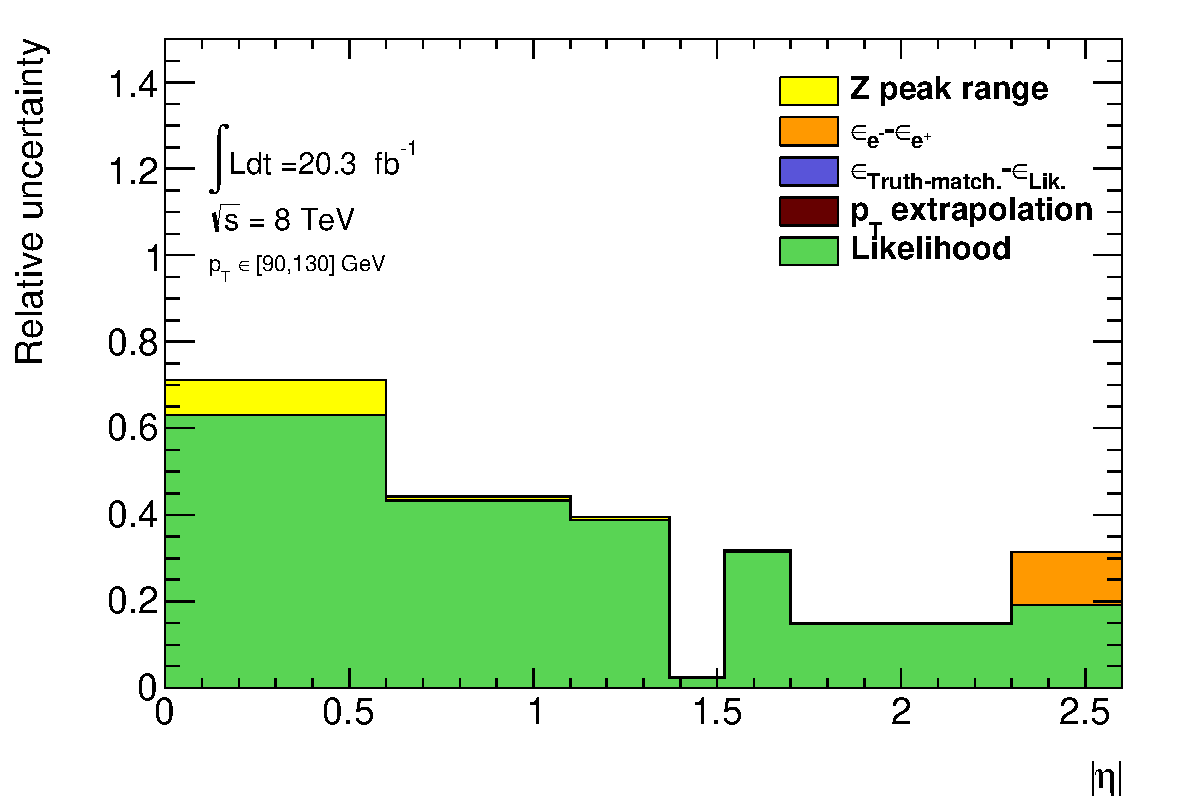
\includegraphics[width=0.48\textwidth]{figs/qmis/Syst3}}% hspace{2cm}%
\fbox{  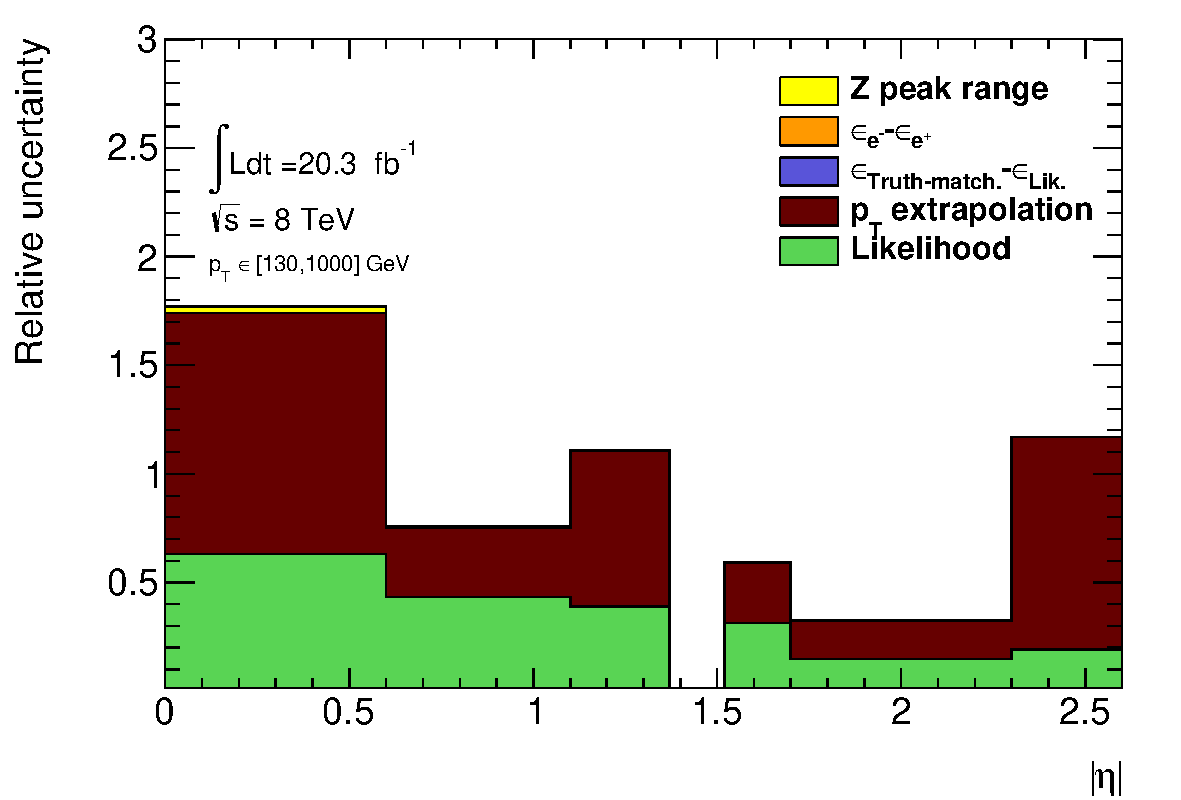
\includegraphics[width=0.48\textwidth]{figs/qmis/Syst4}}% 
\caption{Relative systematic uncertainty contributions on the
      charge mis-identification rate, for different bins in $p_{\rm T}$ and 
      $|\eta|$. Tight++  electrons have been used to produce this plot.}\label{figure:background_qmissyst}
 \end{figure}




We apply the rates to estimate the charge mis-identification background in the 2l SS signal regions, and find  $\sim$ 25\% contamination in the \ee regions and a $\sim$ 10\% contribution to the \emu regions with a 10\% systematic error overall. The low overall error can be attributed to the fact that the statistical error is lowest where the bulk of charge misidentifications occur.  


\section{Fake Lepton Backgrounds}

Fake Leptons, from the mis-identification of jets as either electrons or muons, primarly arise from \ttbar events in the 2l SS, 3l and 4l channels. Smaller contributions come from $Z$+jet events. These backgrounds are sub-dominant but important in the 2lSS and 3l channels but extremely small in the 4l channels. To estimate these backgrounds, we employ data-driven control regions near the signal region with fewer jets that are fake enriched and control regions with reversed cuts. These regions are studied using MC and are shown to be good models for fake backgrounds in the signal region, because they possess similar fake origin and composition. These truth studies suggest that both electrons and muons arise overwhelimingly from  b-quark originated jets.


The general method for all channels is to define a reversed object selection region (usually isolation) for each lepton flavor with otherwise identical signal region selection ($N^e_{CR}$, $N^{\mu}_{CR}$). This region is fake-dominated with small contributions from prompt backgrounds, which are subtracted from the data. The total number of fake events in this region is then scaled by a transfer factor ($\theta$) to estimate the number of fake events of the appropriate flavor in the siganl region. The transfer factor is defined in Equations \ref{equation:background_theta} and the simple formula for determining fakes is defined in Equations \ref{equation:background_total}. 'x' refers to any combination of tight muons and/or electrons, 'd' refers to anti-identified electrons, and 'p' refers to anti-identified muons.  


\begin{equation}
\theta_e = \frac{N_{xe}}{N_xd}, \theta_{\mu} = \frac{N_{x\mu}}{N_{xp}}
\label{equation:background_theta}
\end{equation}

\begin{equation}
N_{fake} = \theta_e * N^e_{CR} + \theta_{\mu} * N^{\mu}_{CR}   
\label{equation:background_total}
\end{equation}


This approach factorizes the background model into two separate measurements. $N_{CR}$ is sensitive the overall \ttbar production rate, especially in the presence of additional jets from QCD ratio, as well as the object-level misidentification of a jet as a lepton. The transfer factor $\theta$ is sensitive to only the object level properties of the mis-identified jet, and in particular only the variables which are reversed in the anti-tight indentification. 

The transfer factor is obtained in a different way for each channel, due to unique issues with statistics and contamination, but each method relies heavily on the data-based control regions with fewer jets. Figure \ref{figure:background_njetr} shows a truth study of the stability of the transfer factor for the 2l SS and 3l cases as a function of the number of jets in the event for events with one-btagged jet. This suggest that the regions with fewer jets are a good model of the fakes in the signal regions with more jets and is expected because of the homogeneity of origin of the fakes across all jet bins.  

The details of the methods for each channel are discussed in depth in the following sections. For all methods, the overall systematic uncertainty on the normalization of the fake estimate is in the range 30\%-50\% and arise primarly from statistics and the closure on assumptions used to obtain the transfer factor.

\begin{figure}[htbp]
\begin{minipage}[h]{0.5\textwidth}
    \centering 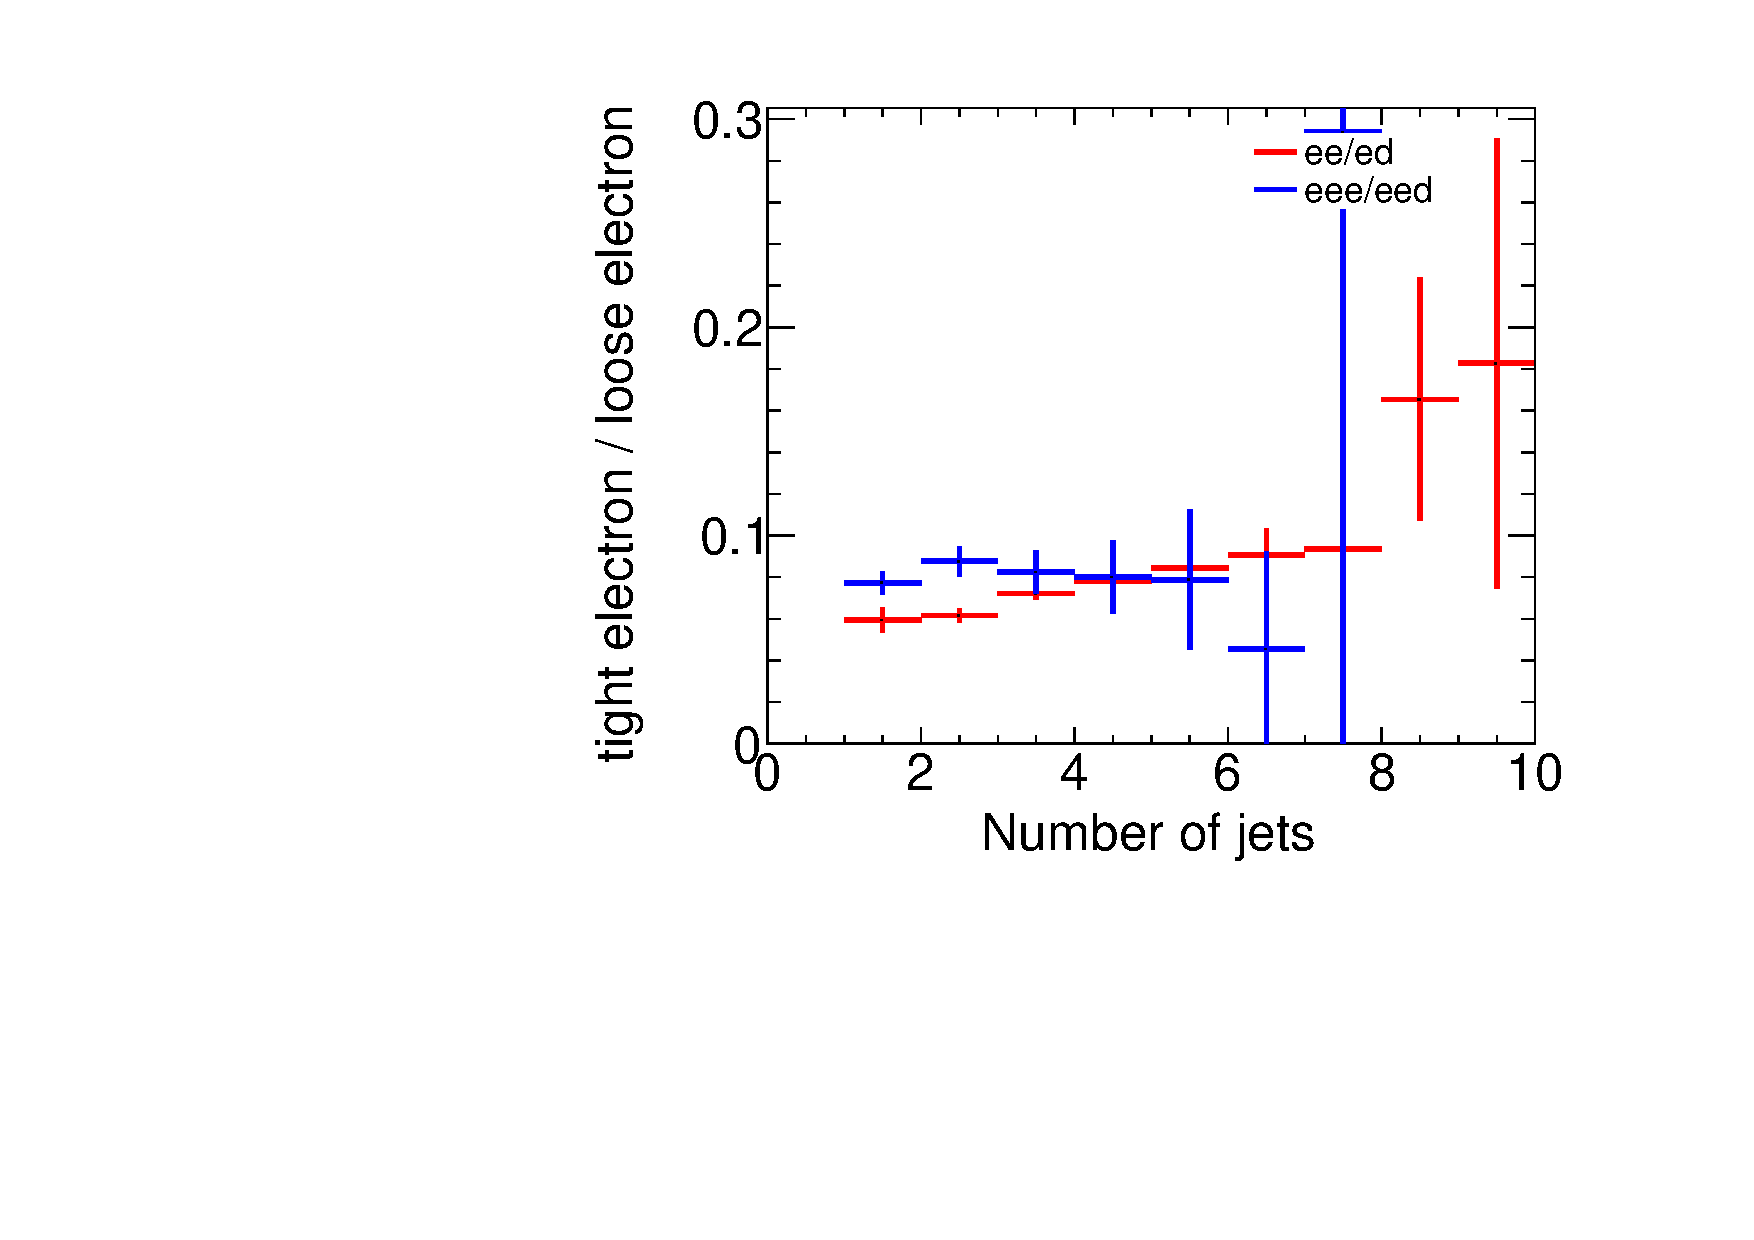
\includegraphics[width=\textwidth]{figs/fake/compare_2e_3e_NJet_ratios}
\end{minipage}\hfill
\begin{minipage}[h]{0.5\textwidth}
    \centering 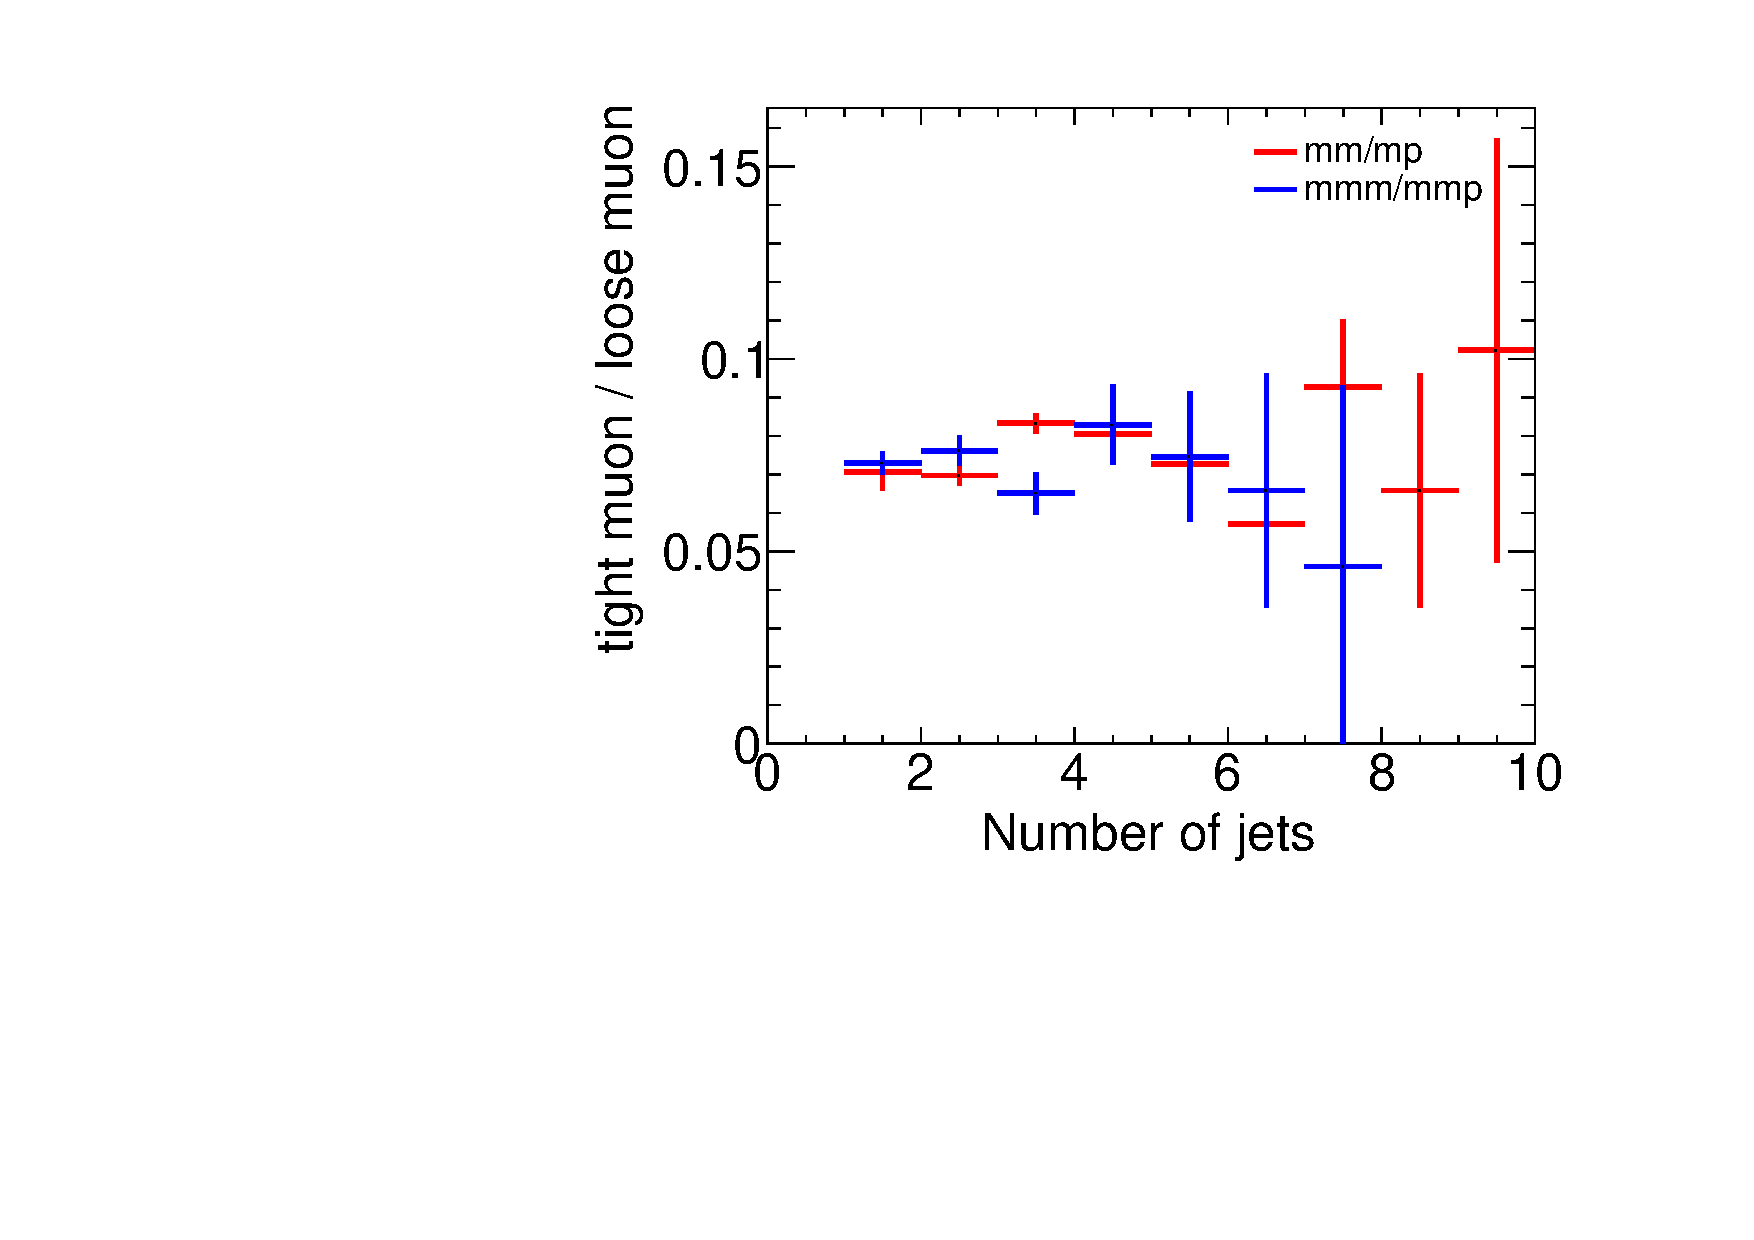
\includegraphics[width=\textwidth]{figs/fake/compare_2m_3m_NJet_ratios}
\end{minipage}\hfill
\caption{Ratios of regions with tight and loose leptons in 2-lepton and 3-lepton channels}
\label{figure:background_njetr}
\end{figure}

Because these methods do provide a per-object transfer-factor that depends on the properties of the faking object, we must use the MC to model the shapes of the fake kinematic distributions in the signal regions. This is not an essential issue, since the analysis only cconsiders only the total number of events in each signal region in the final measurement of \tth production.

\subsection{2l SS Fakes}
The 2l SS fake method follows the procedure outlined in general above. We define anti-tight electron and muon control regions with reversed particle identification criteria for each signal region, including the 6 flavor and jet-counting sub regions. The anti-tight muon and electron criteria are provided below:
  
\begin{itemize}

\item {\bf electron}: fails to verify the {\textsc verytight} likelihood operating point, but still verifies the {\textsc veryloose} opoperating point. fails relative tracking and calorimeter isolation, $\rm E_{T}^{rel}>0.05$ and $\rm p_{T}^{rel}>0.05$.

\item {\bf muon}: 6 \gevc $<$ \pt\ $<$ 10 \gevc

\end{itemize}

The electron and muon transfer factors, $\theta_e$ and $\theta_{\mu}$, are calculated in the region with signal region selection but fewer jets, $NJet == 2$ or $NJet ==3$ and are defined as the ratio of the number of events for two fully identified leptons to the number of events with one fully identified lepton and one anti-identified lepton, after the prompt and charge mis-identification bakgrounds are subtracted. Only same-flavor channels are used to ensure that muon and electron transfer factors maybe estimated separately:
on every region, the prompt and charge-misidentification backgrounds are subtracted from the data. 

 \begin{equation}
 \theta_{e} = \frac{N_{ee}}{N_{ed}}= \frac{  N^{Data}_{ee} - N^{\rm
 Prompt~SS}_{ee} - N^{\rm QMisId}_{ee} }{ N_{ed}^{Data} - N^{\rm
 Prompt~SS}_{ed} - N^{\rm QMisId~MC}_{ed} } 
\end{equation}
\label{equation:ss_def_thee}


 \begin{equation}
 \theta_{m} = \frac{N_{\mu\mu}}{N_{\mu p}}= \frac{ N_{\mu\mu}^{Data} - N^{\rm
 Prompt~SS}_{\mu\mu}}{ N_{\mu p}^{Data} - N^{\rm
 Promt~SS}_{\mu p} } 
\end{equation}
\label{equation:ss_def_thmm}

Figures show the plots of NJet used for the regions used in the transfer factor extrapolation. Other kintematic distributions
  are not shown for brevity




 % Figures

 % Results 

 % Errors 

  % Needs to be updated by Djamel




\subsection{3l Fakes}

The 3l fake method follows the same general strategy as above. Hoewver, the low NJet region has too low statistics


\subsection{4l Fakes}
